\documentclass[12pt,a4paper]{book}
\usepackage[utf8]{inputenc}
\usepackage[spanish,es-tabla]{babel}
\usepackage{amsmath}
\usepackage{amsfonts}
\usepackage{amssymb}
\usepackage{makeidx}
\usepackage{graphicx}
\usepackage{lmodern}
\usepackage{hyperref}
\usepackage{subcaption}
\usepackage{pgfplots}
\pgfplotsset{width=10cm,compat=1.9}
\usepgfplotslibrary{external}
\tikzexternalize

\setlength{\parindent}{0px}
\usepackage[left=2cm,right=2cm,top=4cm,bottom=2cm]{geometry}

\author{Daniel Vázquez Lago, Grupo Nº 6, Pareja Nº8}
\begin{document}

\title{Tecnicas experimentales I: laboratorio básico}
\maketitle
\tableofcontents

\chapter{Introducción a la propagación de incertidumbres}\label{Ch:introduccion-incertidumbres}\newpage
En este capítulo veremos las diferentes ecuaciones que usaremos a lo  largo de todas las prácticas de manera repetida. De esta forma quedarán definidas todas las fórmulas y no será necesario mencionarlas cada vez que las usemos en cada práctica ,ahorrando así bastante tiempo y espacio. Si el lector ya las conoce recomendamos que salte esta parte, ya que es un mero anexo para que se entienda de donde proceden todos nuestros valores. \\

\section{Medidas directas}
Si tomamos varias medidas con la misma precisión (y aparato) tenemos que podemos obtener un valor haciendo la media de dichas medidas. La media es la suma de todas las medidas entre el número de medidas que has tomado. De forma rigurosa se define como el valor más probable que tenga el dato real si suponemos que la muestra de medidas describe una distribución normal. Si tenemos que las medidas $x_i$ con $i=1,2,...,n$ tendremos que:
\begin{equation}
\bar{x}=\dfrac{\sum_{i=1}^n x_i}{n}
\label{Ec: valor medio o media}
\end{equation}
La incertidumbre de la muestra mediante la evaluación de tipo A (i.e. sin tener en cuenta la precisión de las medidas) llamada \textbf{desviación típica} o $s_A (x)$ viene dada por:
\begin{equation}
s_A(x) = \sqrt{\dfrac{\sum_{i=1}^n (x_i - \bar{x})^2}{n-1}}
\label{Ec: desviación estandar de la muestra}
\end{equation}
Y la \textbf{desviación típica de la media} viene dada por:
\begin{equation}
s_A(\bar{x}) = \dfrac{s_A(x)}{\sqrt{n}}
\label{Ec: desviación estandar de la media}
\end{equation}
Sin embargo estamos ignorando la precisión propia de las diferentes medidas, la cual realmente influye en la incertidumbre del valor medio. Como la precisión para todas las medidas es la misma (y no existe peso relativo) podemos usar la siguiente fórmula para calcular la \textbf{incertidumbre combinada} que es la que realmente usamos al describir la incertidumbre del valor medio. Esta se define como:
\begin{equation}
s_C(\bar{x})=\sqrt{[s_A(\bar{x})]^2+[s_B (\bar{x})]^2}
\label{Ec: desviación combinada de la media}
\end{equation}
Siendo $s_B$ la incertidumbre de cada una de las medidas que usamos. 

\section{Medidas indirectas}
Cuando queremos calcular la incertidumbre de una magnitud que deriva de otras , de las cuales si que conocemos su incertidumbre, tenemos que aplicar la fórmula conocida como \textbf{ecuación general de propagación de incertidumbres}. Sea $y$ la magnitud derivada (de la cual queremos calcular su incertidumbre) y sean $x_1, x_2, ..., x_n$ las magnitudes de las que deriva. Si se relacionan a través de la función $y=f(x_1, x_2,...,x_n)$ tendremos que la incertidumbre de y será:
\begin{equation}
s(y)= \sqrt{ \sum_{i=1}^{n} (\dfrac{\partial y}{\partial x_i})^2 s^2(x_i)}
\end{equation}
\section{Regresión lineal simple}\label{Sec:regresión-lineal-simple}
Aquí se detallarán las fórmulas usadas para calcular la pendiente (b) y el término independiente (a), así como su incertidumbre (s(a), s(b)) y el coeficiente de regresión lineal (r), que es un parámetro que mide la calidad de una regresión lineal:

\begin{equation}
b=\dfrac{n(\Sigma_i x_i y_i)-(\Sigma_i y_i)(\Sigma x_i)}{n(\Sigma x_i^2) -(\Sigma_i x_i)^2}
\label{Ec: ecuación de b regresión lineal simple}
\end{equation}

$ $

\begin{equation}
a=\dfrac{ (\Sigma_i y_i)(\Sigma_i x_i^2)- (\Sigma_i x_i)(\Sigma_i x_iy_i)}{n(\Sigma_i x_i^2)-(\Sigma_i x_i)}
\label{Ec: ecuacion de a regresión lineal simple}
\end{equation}

$ $

\begin{equation}
s=\sqrt{\dfrac{\Sigma_i (y_i-a-bx_i)^2}{n-2}}
\label{Ec: desviación típica del ajuste regresión lineal simple}
\end{equation}

$ $

\begin{equation}
s(b)=s \sqrt{\dfrac{n}{n(\Sigma_i x_i^2)-(\Sigma_i x_i)^2}}
\label{Ec: ecuación incertidumbre de b regresion lineal simple}
\end{equation}

$ $

\begin{equation}
s(a)=s \sqrt{\dfrac{\Sigma_i x_i^2}{n(\Sigma_i x_i^2)-(\Sigma_i x_i)^2} }
\label{Ec: ecuación incertidumbre de a regresión lineal simple}
\end{equation}

$ $

\begin{equation}
r = \dfrac{n (\Sigma_i x_i y_i) - (\Sigma_i x_i)(\Sigma_i y_i)}{\sqrt{[n(\Sigma_i x_i^2)-(\Sigma_i x_i)^2][n(\Sigma_i y_i^2)-(\Sigma_i y_i)^2]}}\label{Ec: coeficiente de regresión lineal simple}
\end{equation}

\subsection{Caso particular: sin término independiente}\label{Sub:regresión-sin-termino-independiente}

En el caso de que la regresión lineal no tenga término independiente (a), por la causa que sea (por ejemplo que la fórmula que se este estudiando no contemple la aparición de un término independiente), tenemos que las fórmulas tanto de la pendiente, su incertidumbre y el coeficiente de regresión lineal cambia:


$ $

\begin{equation}
b=\dfrac{\Sigma_i x_i y_i}{\Sigma x_i^2}
\label{Ec: ecuación de b regresión lineal simple sin término independiente}
\end{equation}

$ $

\begin{equation}
s=\sqrt{\dfrac{\Sigma_i (y_i-bx_i)^2}{n-1}}
\label{Ec: ecuación de la desviación típica del ajuste regresión lineal simple sin término independiente}
\end{equation}

$ $

\begin{equation}
s(b)=\dfrac{s}{\sqrt{\Sigma x_i^2}}
\label{Ec: ecuación de b regresión lineal simple sin término independiente}
\end{equation}

$ $

\begin{equation}
r=\dfrac{\Sigma_i x_i y_i}{\sqrt{(\Sigma x_i^2)(\Sigma x_i^2)}}
\label{Ec: ecuación de b regresión lineal simple sin término independiente}
\end{equation}

%_________________BALANZA ELECTRODINAMICA________________



\chapter{Balanza electrodinámica (borrador)} \newpage
\section{Objetivos e introducción}
El objetivo principal de esta práctica es determinar la dirección y sentido de la fuerza que actúa sobre un conductor por el que circula una corriente bajo la acción de un campo magnético, y como se comporta en función de los siguientes parámetros: la longitud del conductor, la intensidad de la corriente y la intensidad del campo magnético. Además se estudiará cual es la relación entre la intensidad de campo magnético aplicado y la intensidad de corriente que aplicamos a la bobina (ya que dicho campo magnético lo creará una bobina). \\

Como es una práctica-borrador no tenemos introducción teórica, asi que describiré brevemente la fórmula principal que vamos a usar, los parámetros que vamos a calcular... \\

La ley general que vamos a usar es la siguiente, la llamada fuerza de Lorentz:

\begin{equation}
F = I_e \ l \ B
\label{Ec:balanza Fuerza de lorentz}
\end{equation}

Donde $F$ es la fuerza magnética, $I_e$ la corriente de la espira (es decir del conductor), $l$ es la longitud de la espira (a la cual se le aplica la fuerza, ya que si $\vec{l} || \vec{B}$ no hay fuerza) y $B$ el campo magnético, que se relacionará con la intensidad de la bobina de la siguiente forma:

\begin{equation}
B=\mathrm{C} \cdot I_B
\label{Ec:balanza Valor del campo magnético}
\end{equation}

Entonces a lo largo de la práctica trataremos de calcular B (en las dos primeras partes) y de ahí extraer el valor de C; y en la segunda parte la obtendremos directamente. De esta forma obtendremos 12 valores para B y 16 para C
\section{Análisis de datos}

Lo que primero debemos hacer es medir el peso de la espira sin aplicarle ningún tipo de fuerza magnética, ya que la fuerza magnetica tenemos que obtenerla directamente de la diferencia entre la fuerza neta total (cuando aplicamos hay campo magnético) y la fuerza neta total sin campo , es decir, el peso de la espira; siguiendo la siguiente fórmula:


\begin{equation}
F_{mag}=g(P_N-P_0)
\label{Ec:balanza fuerza magnetica espira}
\end{equation}

Siendo multiplicada por $g$ ya que la \textbf{balanza} que usamos mide la fuerza en kilopondios (kp), no la fuerza en Newtons. Además la precisión será de 0,01 mkp; y por lo tanto la incertidumbre de $P_N$ y $P_0$ también será de 0,01 mkp. \\

Para no tener que calcular constantemente $P_0$ cada vez que vayamos a tomar una medida, lo que haremos para agilizar el proceso será tomar 5 veces de forma independiente el peso de las espiras, para luego hacer una media, y tomar dicho valor para el resto de la práctica. En la siguiente tabla se representan dichos valores, siendo la ultima fila los valores finales que usaremos con la incertidumbre (combinada): \\ \newpage

\vspace*{1.0cm}

\begin{table}[h!]
\begin{center}
\begin{tabular}{|c|c|c|c|c|}
\hline
Medida & 	$P_0$  (l=12,5mm) & $P_0$	 (l=25mm) & $P_0$	 (l=50mm) & 	$P_0$  (l=100mm) \\  \hline
1 & 	 31,46 & 	 31,97 & 	 38,50 & 	 36,2 \\
2 & 	 31,41 & 	 32,05 & 	 38,61 & 	 36,26 \\
3 & 	 31,43 & 	 32,03 & 	 39,50 & 	 36,28 \\
4 & 	 31,47 & 	 31,82 & 	 38,37 & 	 36,17 \\
5 & 	 31,50 & 	 31,84 & 	 38,52 & 	 36,21 \\  \hline
$\bar{x_0}$ & 	 31,45 $\pm 0,019 $& 	 31,94 $\pm 0,049$ & 	 $38,70 \ \pm 0,20$ & 	 36,22 $\pm 0,022$ \\
\hline
\end{tabular}
\caption{peso para cada espira sin campo magnético ($\bar{x_0}=\bar{P_0}$)}
\label{tab:balanza medias del peso de las espiras sin campo Balanza electrodinamica}
\end{center}
\end{table}

\vspace*{0.5cm}


Como se puede observar para l=50mm hay un dato que se sale de la incertidumbre, por lo que podemos eliminarlo y calcular de nuevo la media y la incertidumbre, que será $P_0=38,5 \pm 0,040 g$. Esto se debe a que 39,4 $\notin$ (38,5-0,20 , 38,5+0,20) \\.

Por lo tanto la incertidumbre de la fuerza magnética vendrá dada por la siguiente fórmula:

\begin{equation}
s(F_{mag})=\sqrt{g^2(s(P_N))^2+g^2(s(P_0))^2}
\label{Ec:balanza incertidumbre de la fuerza magnetica balanza electrodinamica}
\end{equation}

\vspace*{0.10cm}


Tomando los siguientes valores, ya que las incertidumbres serán constantes para cada valor:

\begin{table}[h!]
\begin{center}
\begin{tabular}{|c|c|c|c|}
\hline
$s(P_{mag}) $ (mkp) (l=12,5mm) & $s(P_{mag})$ (mkp) (l=25mm) & $s(P_{mag})$ (mkp) (l=50mm) & $s(P_{mag})$ (mkp) (l=100mm) \\ \hline
0,20 & 0,44 & 0,40 & 0,22 
\\ \hline
\end{tabular}
\end{center}
\caption{Incertidumbres de la fuerza magnética para cada espira}
\end{table}

Además de esto también explicaremos como obtendremos el valor de la constante a partir de $I_B$, ya que usaremos dichas ecuaciones para las dos primeras partes de la práctica. Como ya dijimos el campo magnético se obtiene de multiplicar la intensidad que circula por la bobina por un valor que llamaremos C. Dicho valor se puede obtener si conocemos tanto $B$ como $I_B$, por lo que:


\begin{equation}
\mathrm{C}=\dfrac{B}{I_B}
\label{Ec:balanza Valor de la constante Balanza electrodinamica}
\end{equation}

Y por lo tanto su incertidumbre vendrá dada por:

\begin{equation}
s(\mathrm{C})=\sqrt{(\dfrac{1}{I_B})^2(s(B))^2+(\dfrac{B}{I_B^2})^2(s(I_B))^2}
\label{Ec:balanza valor de la constante Balanza electrodinamica incertidumbre}
\end{equation}

\newpage


\subsection{Fuerza magnética versus intensidad de las espiras (regresión hecha a mano)}


\vspace*{0.5cm}

En esta parte lo que haremos será ir viendo cual es el valor de la fuerza magnética en función del valor de la intensidad que recorra a la espira ($I_e$); dejando tanto $l$ como $B$ constantes a lo largo de la práctica. Entonces si realizamos una regresión lineal que nos permita relacionar $I_e$ y $F_{mag}$ de tal forma que:

$$ F_{mag}=b \cdot I_e $$


\vspace*{0.10cm}

Entonces teniendo en cuenta la ecuación \ref{Ec:balanza Fuerza de lorentz} podemos deducir que:

$$ B \cdot l = b $$

\vspace*{0.10cm}


Y que entonces podemos despejar $B$ obteniendo los siguientes valores:


\begin{equation}
B=\dfrac{b}{l}
\label{Ec: valor de cte con Ie constante balanza electrodnamica}
\end{equation}

\vspace*{0.10cm}


Teniendo en cuenta que su incertidumbre viene dada por:

\begin{equation}
s(B)=\sqrt{(\dfrac{1}{l})^2s^2(b)}
\label{Ec: incertidumbre de cte con Ie constante balanza electrodnamica}
\end{equation}

\vspace*{0.10cm}


Obtenido ya $B$ y $s(B)$, como a lo largo de la práctica usaremos que:

$$ I_B = 1 A, \ \ s(I_B)=0,05 A$$

\vspace*{0.10cm}


Podremos obtener el valor de C y s(C) teniendo en cuenta las anteriores ecuaciones (véase \ref{Ec:balanza valor de la constante Balanza electrodinamica incertidumbre}). \\

La siguientes prácticas se han realizado a mano todas, aunque por cuestión de eficiencia solo representaremos en estas memorias una. Por eso aparece un parámetro más, s. Las ecuaciones que vamos a usar se pueden ver en el capítulo \ref{Ch:introduccion-incertidumbres} en la subsección \ref{Sub:regresión-sin-termino-independiente}. Calcularemos una regresión lineal simple por dos motivos principalmente: las incertidumbres tanto de $x_i$ ($I_e$) y de $y_i$ ($F_{mag}$) son constantes para todos los valores obtenidos y además s(y)$>$s(x). Tampoco calcularemos el término independiente porque en la fórmula \ref{Ec:balanza Fuerza de lorentz} no aparece ningún término independiente. Además si calculáramos una con término independiente sería tan pequeño que podríamos despreciarlo. Tras esta explicación daremos paso al procedimiento, obteniendo los siguientes valores para l=12,5mm:

\newpage

\vspace*{4.5cm} 

\begin{table}[h!]
\begin{center}
\begin{tabular}{|c|c|c|c|}
\hline
$I_B  \pm 0,05 \ \  (A)$ & 	 $I_e \pm 0,1 \ \ (A) $ & 	 P$ \pm 0,01\ \ (mkp)$ & 	 $F_{mag} \pm 0,20 \ \ (N)$ \\  \hline
1,00 & 	 0,2 & 	 31,55 & 	 0,94 \\
1,00 & 	 0,4 & 	 31,65 & 	 1,92 \\
1,00 & 	 0,6 & 	 31,72 & 	 2,61 \\
1,00 & 	 0,8 & 	 31,85 & 	 3,88 \\
1,00 & 	 1,0 & 	 31,94 & 	 4,77 \\
1,00 & 	 1,2 & 	 32,00 & 	 5,36 \\
1,00 & 	 1,4 & 	 32,09 & 	 6,24 \\
1,00 & 	 1,6 & 	 32,12 & 	 6,53 \\
1,00 & 	 1,8 & 	 32,18 & 	 7,12 \\
1,00 & 	 2,0 & 	 32,24 & 	 7,71 \\
1,00 & 	 2,2 & 	 32,27 & 	 8,00 \\
1,00 & 	 2,4 & 	 32,32 & 	 8,50 \\
1,00 & 	 2,6 & 	 32,35 & 	 8,79 \\
1,00 & 	 2,8 & 	 32,42 & 	 9,48 \\
1,00 & 	 3,0 & 	 32,45 & 	 9,77 \\
1,00 & 	 3,2 & 	 32,49 & 	 10,16 \\
1,00 & 	 3,4 & 	 32,54 & 	 10,65 \\
1,00 & 	 3,6 & 	 32,56 & 	 10,85 \\
1,00 & 	 3,8 & 	 32,64 & 	 11,63 \\
1,00 & 	 4,0 & 	 32,67 & 	 11,93 \\
\hline
\end{tabular}
\end{center}
\caption{valores de la fuerza magnética para la espira l=12,5mm variando $I_e$}
\end{table}

\newpage


\vspace*{1.5cm} 

\begin{table}[h!]
\begin{center}
\begin{tabular}{|c|c|c|c|c|c|c|c|}
\hline 
i & 	 $x_i$ & 	 $y_i$ & 	 $x_i^2$ & 	 $y_i^2$ & 	 $x_i \cdot y_i$ & 	 $ y_i-bx_i $ & 	 $(y_i-bx_i)^2$
  	\\  \hline
1 & 	 0,2 & 	 0,94 & 	 0,04 & 	 0,89 & 	 0,19 & 	 0,28 & 	 0,08
  	\\ 
2 & 	 0,4 & 	 1,92 & 	 0,16 & 	 3,70 & 	 0,77 & 	 0,60 & 	 0,36
  	\\ 
3 & 	 0,6 & 	 2,61 & 	 0,36 & 	 6,81 & 	 1,57 & 	 0,62 & 	 0,38
  	\\ 
4 & 	 0,8 & 	 3,88 & 	 0,64 & 	 15,09 & 	 3,11 & 	 1,23 & 	 1,52
  	\\ 
5 & 	 1,0 & 	 4,77 & 	 1,00 & 	 22,73 & 	 4,77 & 	 1,45 & 	 2,11
  	\\ 
6 & 	 1,2 & 	 5,36 & 	 1,44 & 	 28,69 & 	 6,43 & 	 1,38 & 	 1,90
  	\\ 
7 & 	 1,4 & 	 6,24 & 	 1,96 & 	 38,93 & 	 8,73 & 	 1,60 & 	 2,55
  	\\ 
8 & 	 1,6 & 	 6,53 & 	 2,56 & 	 42,69 & 	 10,45 & 	 1,23 & 	 1,51
  	\\ 
9 & 	 1,8 & 	 7,12 & 	 3,24 & 	 50,72 & 	 12,82 & 	 1,15 & 	 1,33
  	\\ 
10 & 	 2,0 & 	 7,71 & 	 4,00 & 	 59,45 & 	 15,42 & 	 1,08 & 	 1,16
  	\\ 
11 & 	 2,2 & 	 8,00 & 	 4,84 & 	 64,08 & 	 17,61 & 	 0,71 & 	 0,50
  	\\ 
12 & 	 2,4 & 	 8,50 & 	 5,76 & 	 72,17 & 	 20,39 & 	 0,54 & 	 0,29
  	\\ 
13 & 	 2,6 & 	 8,79 & 	 6,76 & 	 77,26 & 	 22,85 & 	 0,17 & 	 0,03
  	\\ 
14 & 	 2,8 & 	 9,48 & 	 7,84 & 	 89,80 & 	 26,53 & 	 0,19 & 	 0,04
  	\\ 
15 & 	 3,0 & 	 9,77 & 	 9,00 & 	 95,47 & 	 29,31 & 	 -0,18 & 	 0,03
  	\\ 
16 & 	 3,2 & 	 10,16 & 	 10,24 & 	 103,29 & 	 32,52 & 	 -0,45 & 	 0,20
  	\\ 
17 & 	 3,4 & 	 10,65 & 	 11,56 & 	 113,50 & 	 36,22 & 	 -0,62 & 	 0,39
  	\\ 
18 & 	 3,6 & 	 10,85 & 	 12,96 & 	 117,72 & 	 39,06 & 	 -1,09 & 	 1,18
  	\\ 
19 & 	 3,8 & 	 11,63 & 	 14,44 & 	 135,37 & 	 44,21 & 	 -0,97 & 	 0,93
  	\\ 
20 & 	 4,0 & 	 11,93 & 	 16,00 & 	 142,30 & 	 47,72 & 	 -1,34 & 	 1,78
  	\\  \hline
$\Sigma _i$ & 	 42 & 	 146,86 & 	 114,8 & 	 1280,65 & 	 380,69 & 	 7,58 & 	 18,26
  	\\ 
\hline 
\end{tabular}
\end{center}
\caption{tabla con los valores calculados a mano necesarios para la regresión lineal}
\end{table}



\begin{table}[h!]
\begin{center}
\begin{tabular}{|c|c|c|c|}
\hline
r & 	 b  (mN/A) & 	 s & 	 s(b)  (mN/A) \\ \hline
0,992 & 	 3,3161 & 	 0,98 & 	 0,0085 \\
\hline
\end{tabular}
\end{center}
\caption{valores de b, s(b) y r para la regresión $F_{mag}$ vs $I_e$ para l=12,5mm}
\end{table}

Una vez hecho esto haremos lo mismo para l=25mm, l=50mm y l=100mm, obteniendo las siguientes tablas:

\newpage


\vspace*{3cm} 

\begin{table}[h!]
\begin{center}
\begin{tabular}{|c|c|c|c|}
\hline
$I_B  \pm 0,05 \ \  (A)$ & 	 $I_e \pm 0,1 \ \ (A) $ & 	 $P \pm 0,01\ \ (mkp)$ & 	 $F_{mag} \pm 0,44 \ \ (mN)$ \\ \hline
1,00 & 	 0,2 & 	 32,07 & 	 1,26 \\
1,00 & 	 0,4 & 	 32,22 & 	 2,73 \\
1,00 & 	 0,6 & 	 32,3 & 	 3,51 \\
1,00 & 	 0,8 & 	 32,45 & 	 4,98 \\
1,00 & 	 1,0 & 	 32,57 & 	 6,16 \\
1,00 & 	 1,2 & 	 32,61 & 	 6,55 \\
1,00 & 	 1,4 & 	 32,71 & 	 7,53 \\
1,00 & 	 1,6 & 	 32,83 & 	 8,71 \\
1,00 & 	 1,8 & 	 32,95 & 	 9,89 \\
1,00 & 	 2,0 & 	 33,05 & 	 10,87 \\
1,00 & 	 2,2 & 	 33,16 & 	 11,95 \\
1,00 & 	 2,4 & 	 33,26 & 	 12,93 \\
1,00 & 	 2,6 & 	 33,41 & 	 14,40 \\
1,00 & 	 2,8 & 	 33,50 & 	 15,28 \\
1,00 & 	 3,0 & 	 33,60 & 	 16,26 \\
1,00 & 	 3,2 & 	 33,73 & 	 17,54 \\
1,00 & 	 3,4 & 	 33,83 & 	 18,52 \\
1,00 & 	 3,6 & 	 33,93 & 	 19,50 \\
1,00 & 	 3,8 & 	 34,05 & 	 20,68 \\
1,00 & 	 4,0 & 	 34,15 & 	 21,66 \\
\hline
\end{tabular}
\end{center}
\caption{valores de la fuerza magnética para la espira l=25mm variando $I_e$}
\end{table}


\begin{table}[h!]
\begin{center}
\begin{tabular}{|c|c|c|c|}
\hline
r & 	 b  (mN/A) & 	 s & 	 s(b)  (mN/A) \\ \hline
0,9998 & 	 5,46 & 	 5,3 & 	 0,046 \\
\hline
\end{tabular}
\end{center}
\caption{valores de b, s(b) y r para la representación $F_{mag}$ vs $I_e$ para l=25mm}
\end{table} 

\newpage


\vspace*{2.5cm} 


\begin{table}[h!]
\begin{center}
\begin{tabular}{|c|c|c|c|}
\hline
$I_B  \pm 0,05 \ \  (A)$ & 	 $I_e \pm 0,1 \ \ (A) $ & 	 P$\pm 0,01\ \ (kp)$ & 	 $F_{mag} \pm 0,40 \ \ (mN)$ \\ \hline
1,00 & 	 0,2 & 	 38,75 & 	 2,45 \\ 
1,00 & 	 0,4 & 	 38,94 & 	 4,32 \\ 
1,00 & 	 0,6 & 	 39,15 & 	 6,38 \\ 
1,00 & 	 0,8 & 	 39,38 & 	 8,63 \\ 
1,00 & 	 1,0 & 	 39,55 & 	 10,30 \\ 
1,00 & 	 1,2 & 	 39,74 & 	 12,16 \\ 
1,00 & 	 1,4 & 	 39,98 & 	 14,52 \\ 
1,00 & 	 1,6 & 	 40,19 & 	 16,58 \\ 
1,00 & 	 1,8 & 	 40,25 & 	 17,17 \\ 
1,00 & 	 2,0 & 	 40,45 & 	 19,13 \\ 
1,00 & 	 2,2 & 	 40,64 & 	 20,99 \\ 
1,00 & 	 2,4 & 	 40,81 & 	 22,66 \\ 
1,00 & 	 2,6 & 	 41,05 & 	 25,02 \\ 
1,00 & 	 2,8 & 	 41,27 & 	 27,17 \\ 
1,00 & 	 3,0 & 	 41,45 & 	 28,94 \\ 
1,00 & 	 3,2 & 	 41,62 & 	 30,61 \\ 
1,00 & 	 3,4 & 	 41,80 & 	 32,37 \\ 
1,00 & 	 3,6 & 	 42,03 & 	 34,63 \\ 
1,00 & 	 3,8 & 	 42,22 & 	 36,49 \\ 
1,00 & 	 4,0 & 	 42,42 & 	 38,46 \\ 
\hline
\end{tabular}
\end{center}
\caption{valores de la fuerza magnética para la espira l=50mm variando $I_e$}
\end{table}

\begin{table}[h!]
\begin{center}
\begin{tabular}{|c|c|c|c|}
\hline
r & 	 b  (mN/A) & 	 s & 	 s(b)  (mN/A) \\ \hline
0,9997 & 	 9,6 & 	 15,6 & 	 1,5 \\ 
\hline
\end{tabular}
\end{center}
\caption{valores de la b, s(b) y r para la representación $F_{mag}$ vs $I_e$ para l=50mm}
\end{table} 

\newpage


\vspace*{2.5cm} 


\begin{table}[h!]
\begin{center}
\begin{tabular}{|c|c|c|c|}
\hline
$I_B  \pm 0,05 \ \  (A)$ & 	 $I_e \pm 0,1 \ \ (A) $ & 	 P$\pm 0,01\ \ (kp)$ & 	 $F_{mag} \pm 0,22 \ \ (mN)$ \\ \hline
1,00 & 	 0,2 & 	 36,64 & 	 4,08 \\
1,00 & 	 0,4 & 	 37,05 & 	 8,10 \\
1,00 & 	 0,6 & 	 37,49 & 	 12,42 \\
1,00 & 	 0,8 & 	 37,91 & 	 16,54 \\
1,00 & 	 1,0 & 	 38,35 & 	 20,86 \\
1,00 & 	 1,2 & 	 38,73 & 	 24,58 \\
1,00 & 	 1,4 & 	 39,13 & 	 28,51 \\
1,00 & 	 1,6 & 	 39,53 & 	 32,43 \\
1,00 & 	 1,8 & 	 39,93 & 	 36,36 \\
1,00 & 	 2,0 & 	 40,29 & 	 39,89 \\
1,00 & 	 2,2 & 	 40,67 & 	 43,62 \\
1,00 & 	 2,4 & 	 41,10 & 	 47,83 \\
1,00 & 	 2,6 & 	 41,47 & 	 51,46 \\
1,00 & 	 2,8 & 	 41,90 & 	 55,68 \\
1,00 & 	 3,0 & 	 42,28 & 	 59,41 \\
1,00 & 	 3,2 & 	 42,64 & 	 62,94 \\
1,00 & 	 3,4 & 	 43,02 & 	 66,67 \\
1,00 & 	 3,6 & 	 43,47 & 	 71,08 \\
1,00 & 	 3,8 & 	 43,82 & 	 74,52 \\
1,00 & 	 4,0 & 	 44,17 & 	 77,95 \\
\hline
\end{tabular}
\end{center}
\caption{valores de la fuerza magnética para la espira l=100mm variando $I_e$}
\end{table}

\begin{table}[h!]
\begin{center}
\begin{tabular}{|c|c|c|c|}
\hline
r & 	 b  (mN/A) & 	 s & 	 s(b)  (mN/A) \\ \hline
0,99992 & 	 19,77 & 	 40,5 & 	 0,35 \\
\hline
\end{tabular}
\end{center}
\caption{valores de la b, su s(b) y r para la representación $F_{mag}$ vs $I_e$ para l=100mm}
\end{table}

\newpage

Ahora que hemos obtenido todos los valores de b, s(b) y r construiremos una gráfica enfrentando a $I_e$ vs $F_{mag}$ para cada espira, para que así podamos comparar mejor los resultados:

\begin{figure}[h!] %plot 1 balanza electrodinamica
\centering
\includegraphics[width=11cm, height=7cm]{Plot1-balanzaelectrodinamica.png}
\caption{Representación de $F_{mag}$ vs $I_e$ a $l$ e $I_b$ constantes}
\label{fig:Plot1-balanzaelectrodinamica}
\end{figure}

Una vez obtenimos todos los valores de b, como ya mencionamos anteriormente, obtendremos los valores de B y de su incertidumbre:

\begin{table}[h!]
\begin{center}
\begin{tabular}{|c|c|c|c|c|}
\hline
l  (mm) & 	 b    (mN/A) & 	 s(b)    (mN/A) & 	 B   (T) & 	 s(B)   (T) \\ \hline
12,5 & 	 3,316 & 	 0,092 & 	 0,2653 & 	 0,0073 \\ 
25 & 	 5,46 & 	 0,49 & 	 0,218 & 	 0,020 \\ 
50 & 	 9,6 & 	 1,5 & 	 0,193 & 	 0,029 \\ 
100 & 	 19,8 & 	 3,8 & 	 0,198 & 	 0,038 \\  \hline
\end{tabular}
\end{center}
\caption{valores de B y s(B) creado por una bobina donde circula una corriente de 1A }
\label{Tab:balanza-valor-B-Ie}
\end{table}

Y a partir de B y su incertidumbre obtendremos los valores de C:

\begin{table}[h!]
\begin{center}
\begin{tabular}{|c|c|c|c|c|c|}
\hline
l (mm) & 	 B   (T) & 	 s(B)   (T) & 	 $ I_B \ \pm$ 0,05 (A) & 	 C (T/A) & 	 s(C) (T/A) \\  \hline
12,5 & 	 0,2653 & 	 0,0073 & 	 1 & 	 0,265 & 	 0,015 \\ 
25 & 	 0,218 & 	 0,020 & 	 1 & 	 0,218 & 	 0,022 \\ 
50 & 	 0,193 & 	 0,029 & 	 1 & 	 0,193 & 	 0,031 \\ 
100 & 	 0,198 & 	 0,038 & 	 1 & 	 0,198 & 	 0,039 \\ 
\hline
\end{tabular}
\end{center}
\caption{valores de la constante (C) que relaciona $I_B$ con B (y su incertidumbre)}
\label{Tab:balanza-valor-cte-Ie}
\end{table}

\newpage


\subsection{Fuerza magnética versus longitud de las espiras}
En esta parte veremos como varía $F_{mag}$ a $I_e$ y $B$ constante en función de que espira cojamos (es decir, en función de l). Para esto usaremos valores anteriores, es decir, cogeremos los valores de $I_e=0,8A; \ 1,6A...$ hasta $4A$, de cada una de la espiras y veremos la dependencia lineal en función de la la longitud l. De esta forma, al igual que antes, haremos una regresión lineal que nos permitirá calcular la pendiente que relacione $l$ y $F_{mag}$:

$$ F_{mag} = b \cdot l  $$

Por lo que:

$$ b = B \cdot I_e $$

Y despejando B:

\begin{equation}
B=\dfrac{b}{I_e}
\label{Ec: valor de cte con l constante balanza electrodinamica}
\end{equation}

Siendo su incertidumbre:

\begin{equation}
s(B)=\sqrt{(\dfrac{b}{I_e^2})^2s^2(I_e)+(\dfrac{1}{I_e})^2s^2(b)}
\label{Ec: incertidumbre de cte con l constante balanza electrodnamica}
\end{equation}

Hecho esto podremos obtener los valores de C y s(C) aplicando las fórmulas anteriores.  \\

El principal problema que tiene esta forma de proceder es que la incertidumbre de $F_{mag}$ va variando en función de cual cojamos. De todos modos como la variación entre el valor mínimo y máximo es despreciable (no llega a un orden de diferencia), no tendremos en cuenta esta variación. Por ello realizaremos una regresión lineal simple. Además será sin término independiente, por las mimas razones que hemos citado para el apartado anterior. \\

Ahora sí, tomando los datos anteriores y agrupándolos en una tabla para facilitar los cálculos y la visualización de los resultados:


\vspace*{1.0cm} 

\begin{table}[h!]
\begin{center}
\begin{tabular}{|c|c|c|c|c|}
\hline
$ l \ \ (mm) $ & 	 $ I_e \pm 0,1 \ (A) $ & 	 P$\pm 0,01\ \ (mkp)$ & 	 $F_{mag} \ (mN)$ & 	 $s(F_{mag}) \ (mN)$ \\ \hline
12,5 & 	 0,8 & 	 31,85 & 	 3,88476 & 	 0,20 \\ 
25 & 	 0,8 & 	 32,45 & 	 4,98348 & 	 0,44 \\ 
50 & 	 0,8 & 	 39,38 & 	 8,6328 & 	 0,40 \\ 
100 & 	 0,8 & 	 37,91 & 	 16,53966 & 	 0,22 \\ 
\hline
\end{tabular}
\label{Tab: Fmag vs l a Ie=0,8A balanza}
\caption{valores de $F_{mag}$ en función de l a $I_B$ e $I_e$ (0,8 A) constantes}
\end{center}
\end{table} \newpage



\vspace*{2.5cm} 

\begin{table}[h!]
\begin{center}
\begin{tabular}{|c|c|c|c|c|}
\hline
$ l \ \ (mm) $ & 	 $ I_e \pm 0,1 \ (A) $ & 	 P$\pm 0,01\ \ (mkp)$ & 	 $F_{mag} \ (mN)$ & 	 $s(F_{mag}) \ (mN)$ \\ \hline
12,5 & 	 1,6 & 	 32,12 & 	 6,53346 & 	 0,20 \\ 
25 & 	 1,6 & 	 32,83 & 	 8,71128 & 	 0,44 \\ 
50 & 	 1,6 & 	 40,19 & 	 16,5789 & 	 0,40 \\ 
100 & 	 1,6 & 	 39,53 & 	 32,43186 & 	 0,22 \\ 
\hline
\end{tabular}
\label{Tab: Fmag vs l a Ie=1,6A balanza}
\caption{valores de $F_{mag}$ en función de l a $I_B$ e $I_e$ (1,6 A) constantes}
\end{center}
\end{table}


\begin{table}[h!]
\begin{center}
\begin{tabular}{|c|c|c|c|c|}
\hline
$ l \ \ (mm) $ & 	 $ I_e \pm 0,1 \ (A) $ & 	 P$\pm 0,01\ \ (mkp)$ & 	 $F_{mag} \ (mN)$ & 	 $s(F_{mag}) \ (mN)$ \\ \hline
12,5 & 	 2,4 & 	 32,32 & 	 8,49546 & 	 0,20 \\ 
25 & 	 2,4 & 	 33,26 & 	 12,92958 & 	 0,44 \\ 
50 & 	 2,4 & 	 40,81 & 	 22,6611 & 	 0,40 \\ 
100 & 	 2,4 & 	 41,1 & 	 47,83356 & 	 0,22 \\ 
\hline
\end{tabular}
\label{Tab: Fmag vs l a Ie=2,4A balanza}
\caption{valores de $F_{mag}$ en función de l a $I_B$ e $I_e$ (2,4 A) constantes}
\end{center}
\end{table}


\begin{table}[h!]
\begin{center}
\begin{tabular}{|c|c|c|c|c|}
\hline
$ l \ \ (mm) $ & 	 $ I_e \pm 0,1 \ (A) $ & 	 P$\pm 0,01\ \ (mkp)$ & 	 $F_{mag} \ (mN)$ & 	 $s(F_{mag}) \ (mN)$ \\ \hline
12,5 & 	 3,2 & 	 32,49 & 	 10,16316 & 	 0,20 \\ 
25 & 	 3,2 & 	 33,73 & 	 17,54028 & 	 0,44 \\ 
50 & 	 3,2 & 	 41,62 & 	 30,6072 & 	 0,40 \\ 
100 & 	 3,2 & 	 42,64 & 	 62,94096 & 	 0,22 \\ 
\hline
\end{tabular}
\label{Tab: Fmag vs l a Ie=3,2A balanza}
\caption{valores de $F_{mag}$ en función de l a $I_B$ e $I_e$ (3,2 A) constantes}
\end{center}
\end{table}


\begin{table}[h!]
\begin{center}
\begin{tabular}{|c|c|c|c|c|}
\hline
$ l \ \ (mm) $ & 	 $ I_e \pm 0,1 \ (A) $ & 	 P$\pm 0,01\ \ (mkp)$ & 	 $F_{mag} \ (mN)$ & 	 $s(F_{mag}) \ (mN)$ \\ \hline 
12,5 & 	 4 & 	 32,67 & 	 11,92896 & 	 0,20 \\ 
25 & 	 4 & 	 34,15 & 	 21,66048 & 	 0,44 \\ 
50 & 	 4 & 	 42,42 & 	 38,4552 & 	 0,40 \\ 
100 & 	 4 & 	 44,17 & 	 77,95026 & 	 0,22 \\ 
\hline
\end{tabular}
\label{Tab: Fmag vs l a Ie=4A balanza}
\caption{valores de $F_{mag}$ en función de l a $I_B$ e $I_e$ (4 A) constantes}
\end{center}
\end{table}

\newpage

En la siguiente figura representamos las 5 regresiones lineales:

\begin{figure}[h!] %plot 3 balanza electrodinamica
\centering
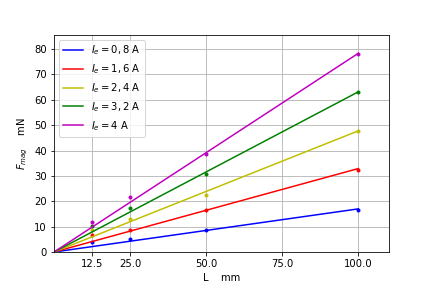
\includegraphics[width=11cm, height=7cm]{plot2-balanzaelectrodinamica.png}
\caption{Representación de $F_{mag}$ vs $l$ a $I_B$ e $I_e$ constantes}
\label{fig:Plot2-balanzaelectrodinamica}
\end{figure}

Una vez hecho esto agrupamos los resultados b, s(b) y r para cada regresión lineal en una sola tabla:

\begin{table}[h!]
\begin{center}
\begin{tabular}{|c|c|c|c|c|}
\hline
$I_e \pm 0,1 \ \  (A)$ & 	 $I_b \pm 0,05 \ \ (A)$ & 	 b  (N/m) & 	 s(b)   (N/m) & 	 r \\ \hline
0,8 & 	 1 & 	 0,17 & 	 0,010 & 	 0,995 \\ 
1,6 & 	 1 & 	 0,33 & 	 0,013 & 	 0,997 \\ 
2,4 & 	 1 & 	 0,48 & 	 0,015 & 	 0,998 \\ 
3,2 & 	 1 & 	 0,63 & 	 0,015 & 	 0,9991 \\ 
4 & 	 1 & 	 0,78 & 	 0,015 & 	 0,9994 \\ 
\hline
\end{tabular}
\caption{valores de b, s(b) y r para las regresiones lineales $F_{mag}$ vs }
\end{center}
\end{table}

De donde podemos extraer B, y posteriormente el valor de C (véase tabla \ref{Tab:balanza-valor-cte--l}):


\begin{table}[h!]
\begin{center}
\begin{tabular}{|c|c|c|c|c|}
\hline
$I_e \pm 0,1 \ \  (A)$ & 	 b    (m/A) & 	 s(b)  (N/A) & 	 B   (T) & 	 s(B)   (T) \\ \hline
0,8 & 	 0,170 & 	 0,010 & 	 0,213 & 	 0,029 \\ 
1,6 & 	 0,329 & 	 0,013 & 	 0,206 & 	 0,015 \\ 
2,4 & 	 0,478 & 	 0,015 & 	 0,199 & 	 0,010 \\ 
3,6 & 	 0,632 & 	 0,015 & 	 0,1755 & 	 0,0064 \\ 
4 & 	 0,784 & 	 0,015 & 	 0,1959 & 	 0,0062 \\ 
\hline
\end{tabular}
\caption{valores de B y s(B) creados por una bobina donde circula una corriente de 1A }
\label{Tab:balanza-valor-B-l}
\end{center}
\end{table}

\newpage

\vspace*{1.0cm}

\begin{table}[h!]
\begin{center}
\begin{tabular}{|c|c|c|c|c|c|}
\hline
$I_e \pm 0,1 \ \  (A)$ & 	 B   (T) & 	 s(B)   (T) & 	$ I_B \pm$ 0,05 (A) & 	 C (T/A) & 	 s(C) (T/A) \\ \hline
0,8 & 	 0,213 & 	 0,029 & 	 1 & 	 0,213 & 	 0,031 \\ 
1,6 & 	 0,206 & 	 0,015 & 	 1 & 	 0,206 & 	 0,018 \\ 
2,4 & 	 0,199 & 	 0,010 & 	 1 & 	 0,199 & 	 0,014 \\ 
3,6 & 	 0,1755 & 	 0,0064 & 	 1 & 	 0,175 & 	 0,011 \\ 
4 & 	 0,1959 & 	 0,0062 & 	 1 & 	 0,196 & 	 0,012 \\ 
\hline
\end{tabular}
\caption{valores de la constante (C y s(C)) que relaciona $I_B$ con B }
\label{Tab:balanza-valor-cte--l}
\end{center}
\end{table}


\vspace*{1.5cm}


\subsection{Fuerza magnética versus intensidad de la bobina}


A diferencia de las dos anteriores partes en esta parte no podremos calcular la intensidad del campo $B$, ya que aquí lo que iremos cambiando es $I_B$. Como sabemos que $B=C \cdot I_B$ podemos substituir esto en la ecuación \ref{Ec:balanza Fuerza de lorentz} de lo que obtenemos:

$$ F_{mag}=C \cdot l \cdot I_e \cdot I_B $$

Por lo tanto si vemos como va variando F en función de $I_B$ obteniendo:

$$ F_{mag}=b \cdot I_B$$

Tenemos que:

$$ b = C \cdot I_e \cdot l$$ 

De donde podemos despejar C obteniendo así la fórmula que usaremos para calcular dicha constante:

\begin{equation}
\mathrm{C}=\dfrac{b}{l \cdot I_e}
\label{Ec: valor de cte con Ib constante balanza electrodinamica}
\end{equation}


\begin{equation}
s(\mathrm{C})=\sqrt{(\dfrac{b}{l \cdot (I_e)^2})^2s^2(I_e)+(\dfrac{1}{l \cdot I_e})^2s^2(b)}
\label{Ec: incertidumbre de cte con Ib constante balanza electrodnamica}
\end{equation}

Al igual que antes realizaremos una regresión lineal simple sin término independiente. Las siguientes tablas muestran los valores obtenidos para cada una de las espiras: 

\newpage

\vspace*{2.5cm}

\begin{table}[h!]
\begin{center}
\begin{tabular}{|c|c|c|c|}
\hline
$I_B  \pm 0,05 \ \  (A)$ & 	 $I_e \pm 0,1 \ \ (A) $ & 	 P$\pm 0,01\ \ (mkp)$ & 	 $F_{mag} \pm 0,20 \ \ (mN)$ \\ \hline
0,1 & 	 4 & 	 31,44 & 	 -0,14 \\
0,2 & 	 4 & 	 31,6 & 	 1,43 \\
0,3 & 	 4 & 	 31,75 & 	 2,90 \\
0,4 & 	 4 & 	 31,87 & 	 4,08 \\
0,5 & 	 4 & 	 31,98 & 	 5,16 \\
0,6 & 	 4 & 	 32,07 & 	 6,04 \\
0,7 & 	 4 & 	 32,2 & 	 7,32 \\
0,8 & 	 4 & 	 32,26 & 	 7,91 \\
0,9 & 	 4 & 	 32,41 & 	 9,38 \\
1 & 	 4 & 	 32,55 & 	 10,75 \\
1,1 & 	 4 & 	 32,63 & 	 11,54 \\
1,2 & 	 4 & 	 32,77 & 	 12,91 \\
1,3 & 	 4 & 	 32,86 & 	 13,79 \\
\hline
\end{tabular}
\label{Tab: Fmag vs IB a l=12,5mm balanza}
\caption{valores de $F_{mag}$ en función de $I_B$ a $I_e$ (4 A) y l (12,5mm) constantes }
\end{center}
\end{table}


\begin{table}[h!]
\begin{center}
\begin{tabular}{|c|c|c|c|}
\hline
$I_B  \pm 0,05 \ \  (A)$ & 	 $I_e \pm 0,1 \ \ (A) $ & 	 P$\pm 0,01\ \ (mkp)$ & 	 $F_{mag} \pm 0,44 \ \ (mN)$ \\ \hline
0,1 & 	 4 & 	 32,22 & 	 2,73 \\
0,2 & 	 4 & 	 32,46 & 	 5,08 \\
0,3 & 	 4 & 	 32,69 & 	 7,34 \\
0,4 & 	 4 & 	 32,9 & 	 9,40 \\
0,5 & 	 4 & 	 33,14 & 	 11,75 \\
0,6 & 	 4 & 	 33,36 & 	 13,91 \\
0,7 & 	 4 & 	 33,55 & 	 15,77 \\
0,8 & 	 4 & 	 33,83 & 	 18,52 \\
0,9 & 	 4 & 	 34,02 & 	 20,39 \\
1 & 	 4 & 	 34,22 & 	 22,35 \\
1,1 & 	 4 & 	 34,46 & 	 24,70 \\
1,2 & 	 4 & 	 34,65 & 	 26,57 \\
1,3 & 	 4 & 	 34,81 & 	 28,14 \\
\hline
\end{tabular}
\label{Tab: Fmag vs IB a l=25mm balanza}
\caption{valores de $F_{mag}$ en función de $I_B$ a $I_e$ (4 A) y l (25mm) constantes }
\end{center}
\end{table}

\newpage

\vspace*{2.5cm}

\begin{table}[h!]
\begin{center}
\begin{tabular}{|c|c|c|c|}
\hline
$I_B  \ pm 0,05 \ \  (A)$ & 	 $I_e \pm 0,1 \ \ (A) $ & 	 P$\pm 0,01\ \ (mkp)$ & 	 $F_{mag} \pm 0,40 \ \ (mN)$ \\ \hline
0,1 & 	 4 & 	 38,94 & 	 4,32 \\ 
0,2 & 	 4 & 	 39,38 & 	 8,63 \\ 
0,3 & 	 4 & 	 39,78 & 	 12,56 \\ 
0,4 & 	 4 & 	 40,21 & 	 16,78 \\ 
0,5 & 	 4 & 	 40,56 & 	 20,21 \\ 
0,6 & 	 4 & 	 40,96 & 	 24,13 \\ 
0,7 & 	 4 & 	 41,39 & 	 28,35 \\ 
0,8 & 	 4 & 	 41,78 & 	 32,18 \\ 
0,9 & 	 4 & 	 42,15 & 	 35,81 \\ 
1 & 	 4 & 	 42,55 & 	 39,73 \\ 
1,1 & 	 4 & 	 42,98 & 	 43,95 \\ 
1,2 & 	 4 & 	 43,43 & 	 48,36 \\ 
1,3 & 	 4 & 	 43,74 & 	 51,40 \\ 
\hline
\end{tabular}
\label{Tab: Fmag vs IB a l=50mm balanza}
\caption{valores de $F_{mag}$ en función de $I_B$ a $I_e$ (4 A) y l (50mm) constantes }
\end{center}
\end{table}


\begin{table}[h!]
\begin{center}
\begin{tabular}{|c|c|c|c|}
\hline
$I_B  \pm 0,05 \ \  (A)$ & 	 $I_e \pm 0,1 \ \ (A) $ & 	 P$\pm 0,01\ \ (mkp)$ & 	 $F_{mag} \pm 0,22 \ \ (mN)$ \\ \hline
0,1 & 	 4 & 	 37,21 & 	 9,67 \\
0,2 & 	 4 & 	 37,98 & 	 17,23 \\
0,3 & 	 4 & 	 38,77 & 	 24,98 \\
0,4 & 	 4 & 	 39,58 & 	 32,92 \\
0,5 & 	 4 & 	 40,34 & 	 40,38 \\
0,6 & 	 4 & 	 41,11 & 	 47,93 \\
0,7 & 	 4 & 	 41,83 & 	 54,99 \\
0,8 & 	 4 & 	 42,65 & 	 63,04 \\
0,9 & 	 4 & 	 43,44 & 	 70,79 \\
1 & 	 4 & 	 44,15 & 	 77,75 \\
1,1 & 	 4 & 	 44,87 & 	 84,82 \\
1,2 & 	 4 & 	 45,64 & 	 92,37 \\
1,3 & 	 4 & 	 46,38 & 	 99,63 \\
\hline
\end{tabular}
\label{Tab: Fmag vs IB a l=100mm balanza}
\caption{valores de $F_{mag}$ en función de $I_B$ a $I_e$ (4 A) y l (100mm) constantes }
\end{center}
\end{table}

\newpage

Los resultados obtenidos de cada una de ellas las agrupamos en una sola tabla:

\begin{table}[h!]
\begin{center}
\begin{tabular}{|c|c|c|c|}
\hline
l  (mm) & 	 b  (mN/A) & 	 s(b) (mN/A) & 	 r \\  \hline
12,5 & 	 10,47 & 	 0,15 & 	 0,998\\ 
25 & 	 22,42 & 	 0,18 & 	 0,9996 \\ 
50 & 	 40,04 & 	 0,15 & 	 0,99992 \\ 
100 & 	 77,91 & 	 0,47 & 	 0,9997 \\  \hline
\end{tabular}
\caption{valores de b, s(b) y r para las regresiones lineales $F_{mag}$ vs $I_B$}
\label{Tab:balanza-valor-b-Ib}
\end{center}
\end{table}



Ahora que tenemos todos los datos necesarios representamos gráficamente las regresiones:

\begin{figure}[h!] %plot 2 balanza electrodinamica
\centering
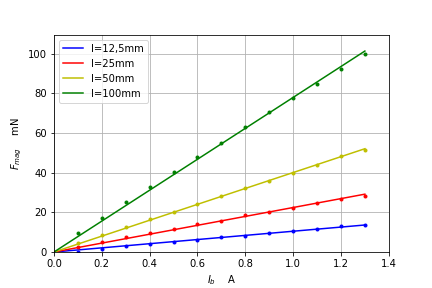
\includegraphics[width=11cm, height=7cm]{plot3-balanzaelectrodinamica.png}
\caption{Representación de $F_{mag}$ vs $i_B$ a $I_e$ e $l$ constantes}
\label{fig:Plot3-balanzaelectrodinamica}
\end{figure}


Y podemos calcular los valores de C:


\begin{table}[h!]
\begin{center}
\begin{tabular}{|c|c|c|c|c|c|}
\hline
l  (mm) & 	 b  (mN/A) & 	 s(b) (mN/A) & 	 $I_e$  $\pm 0,1$   (A) & 	 C (T/A) & 	 s(C) (T/A) \\ \hline
12,5 & 	 10,47 & 	 0,16 & 	 4 & 	 0,2094 & 	 0,0053 \\ 
25 & 	 22,42 & 	 0,18 & 	 4 & 	 0,2242 & 	 0,0056 \\ 
50 & 	 40,04 & 	 0,15 & 	 4 & 	 0,2002 & 	 0,0050 \\ 
100 & 	 77,91 & 	 0,47 & 	 4 & 	 0,1948 & 	 0,0049 \\ 
\hline
\end{tabular}
\caption{valores de la constante (C) que relaciona $I_B$ con B (y su incertidumbre)}
\label{Tab:balanza-valor-cte-Ib}
\end{center}
\end{table}

\newpage

\section{Conclusiones}

Lo primero que debemos hacer es ver si cumplimos los objetivos que nos propusimos, y de ser así, ver si los resultados están bien o muy bien, ver que podemos mejorar, explicar (si hubo) alguna dificultad... \\

En primer lugar: ¿Obtuvimos los valores de B y C? Como se pueden ver en las tablas \ref{Tab:balanza-valor-B-Ie} y \ref{Tab:balanza-valor-B-l} obtuvimos B y su incertidumbre; y en las tablas \ref{Tab:balanza-valor-cte-Ie}, \ref{Tab:balanza-valor-cte--l}, \ref{Tab:balanza-valor-cte-Ib}  obtuvimos C y su incertidumbre. Por lo tanto esta parte el objetivo principal de la práctica está satisfactoriamente realizado. De todos modos vamos a ir un poco mas allá, ya que aun que esten calculados, pueden estar muy mal, con valores muy dispersos entre sí, o incertidumbres sumamente altas. \\

Primero compararemos los valores obtenidos para el campo  magnético B. En general los valores oscilan entre 0,18 T y 0,22 T; lo cual está bastante bien, ya que en general todos dan los mismos valores. Además no estamos teniendo en cuenta las incertidumbres, que en general han sido bastante altas (entre un 10 y 20 \% del valor) ya que tuvimos varios problemas, el mas relevante es que la intensidad de la bobina (que genera el campo magnético) oscilaba mucho, por eso tuvimos que ponerle una incertidumbre relativamente elevada (0,05 A) teniendo en cuenta la precisión del aparato (0,01 A). No solo eso, si no que la fuerza también es bastante difícil de medir, ya que tal y como se miden los datos en la balanza muchas veces dudas si te te dio un valor u otro, ya que la rueda puede estar entre dos valores. De todos modos no es muy precisa, tal y como se puede ver al calcular el peso inicial , en la que divergen muchísimo medidas tomadas en una diferencia de tiempo muy corta con la misma espira (véase \ref{tab:balanza medias del peso de las espiras sin campo Balanza electrodinamica}). Por estas razones obtenemos incertidumbres muy grandes. De todos modos los resultados son todos bastante parecidos, aún teniendo en cuenta las incertidumbres. \\

Sin embargo hay un dato que se va por mucho del rango 0,18 y 0,22 T. Este es el dato obtenido para la espira 12,5mm cuando enfrentamos $F_{mag}$ y $I_e$, dándonos 0,2563 teslas con la incertidumbre más baja de todas las que obtuvimos. ¿Como se explica esto? Pues bien, cuando nosotros hacemos la regresión lineal simple nosotros no tenemos en cuenta el peso relativo de las medidas que cogemos. Lo que quiero decir es que no es lo mismo una incertidumbre de 0,20 mN sobre 11mN que sobre 38mN, y es algo que al calcular s(b) pues no se tiene en cuenta si usamos una regresión lineal. Para evitar esto probablemente lo que tendríamos que hacer es una regresión lineal ponderada, ya que si tiene en cuenta el peso relativo. No es tanto la incertidumbre lo que importa si no la relación dato incertidumbre. Aún así solo es un valor, que si hicieramos una media de B despues descartaríamos ya que se iría del intervalo ($B+s(b), B-s(b)$).\\

A los valores de $I_B$ les sucede lo mismo que $B$, la mayoría (11 de los 12) se encuentran entre 0,18 y 0,22 T/A, y el mismo valor que daba problemas en B (valor de C para la espira l=12,5mm cuando enfrentamos $F_{mag} \mathrm{vs} I_e$); por exactamente las mismas razones. Aquí también hay  unas incertidumbres muy altas, al igual que antes, por que u oscilaban mucho los aparatos, era difícil saber cual eran su valor... De todos modos los valores de C (al igual que B) son muy parecidos entre sí.. \\

Tal y como hemos explicado, los datos, de manera general, se encuentran en los valores que cabrían esperar, y son muy parecidos entre sí, por lo que podríamos considerar está práctica un éxito. Además me gustaría destacar lo bien que salieron las regresiones lineales (esto se puede ver mirando los coeficientes de regresión lineal), muy cercanos a la unidad (siendo el peor 0,992; el cual sigue siendo muy buen dato). Las diferencias entre los coeficientes están causadas por las incertidumbres que hay. Por lo tanto podemos justificar el uso de las regresiones lineales simples; ya que hacerlas de otra forma no cambiaría prácticamente nada los resultados.\\

Todavía yendo un poco más lejos explicaré una dificultad o problema relevante que tuvimos en la práctica. Cuando comencé a realizar está práctica tuvimos un gran problema al calcular el peso inicial y ciertos pesos con fuerza magnética ya que en función de donde coloques la espira (ya que tiene dos ganchos) el valor de F puede cambiar, lo que hizo que apareciera un error sistemático a lo largo de todos los pesos y parte de los otros cálculos. Por ello tuvimos que ir un día después a repetir medidas (donde nos dimos cuenta de ese factor), y por eso muchos datos divergen de los datos que tomamos al principio. \\

Además podemos ver que experimentalmente se cumple la ley de bio-savat, ya que hemos comprobado que tanto l, como B como $I_e$ se relacionan de manera lineal con F. 






%_____________________TENSION SUPERFICIAL__________________




\chapter{Tensión superficial} \newpage

\section{Objetivos}
El objetivo de esta práctica es determinar la tensión superficial de un líquido, que observaremos en diferentes disoluciones de alcohol, en alcohol pura y en agua (a temperatura ambiente) así como varía la tensión superficial en función de la temperatura (usando como líquido el agua). De esta forma calcularemos el coeficiente de tensión superficial para cada medida, y su correspondiente incertidumbre.


\section{Introducción teórica}
Se le llama tensión superficial de un líquido a la fuerza que aparece en la superficie de los líquidos debido a las fuerzas intermoleculares, y que nace al introducir un objeto en el. Las moléculas del líquido se ven afectadas por el sólido, y pueden verse atraídas por las moléculas del sólido. Cuando esto sucede, las moléculas del objeto intentarán mantenerse unidas entre sí (debido a las fuerzas intermoleculares), pero como también estarán atraídas por las moléculas del líquido generará una tensión, que aumentará conforme movemos el sólido tratando de despegarlo del líquido, hasta que finalmente se rompe la película del líquido separando finalmente el objeto. El coeficiente de tensión superficial ($\gamma$)  es una medida de cuanta tensión por unidad de longitud pueden crear este líquido sobre el sólido. 


\begin{figure}[h!]
\centering
\begin{subfigure}[b]{0.4\linewidth}
\includegraphics[scale=0.7]{tensión-imagen1.png}
\caption{representación de las fuerzas}
\label{fig:tension-representacion-fuerzas}
\end{subfigure}
\begin{subfigure}[b]{0.3\linewidth}
\includegraphics[scale=0.6]{tensión-imagen2.png}
\caption{momento en el que F=F'-P}
\label{fig:tensión-punto}
\end{subfigure}
\end{figure}

De este modo podremos calcularlo solo conociendo la longitud del objeto ($L$) que está en contacto con el agua, la masa del mismo ($m$), que multiplicada por $g$ se convertirá en $P$, el peso, y la fuerza que tenemos que ejercer para arrancarlo ($F'$). En nuestro caso el objeto será un disco, por lo que el perímetro en contacto con el agua será $2 \pi d$, ya que tiene dos caras, una interior y otra exterior. La fórmula que relaciona dichos parámetros es:
 
\begin{equation}
F'= 2 \gamma L + P \label{Ec:tension-Fuerza de tensión superficial}
\end{equation}

Entonces el coeficiente de regresión lineal será:

\begin{equation}
\gamma = \dfrac{F'-P}{2L} \label{Ec:tension-Valor de gamma 1}
\end{equation}

Y teniendo en cuenta que $F=F'-P$ y que $L=\pi d$ (siendo d el diametro del disco):

\begin{equation}
\gamma = \dfrac{F}{2\pi d} \label{Ec:tension-Valor de gamma 2}
\end{equation}



\section{Montaje experimental}
En primer lugar mediremos el diámetro de nuestro disco, ya que es una de los parámetros que necesitamos saber. En este caso lo mediremos con una \textbf{regla} de precisión milimétrica, pero que nos parecía poco precisa tomar dicho valor como incertidumbre, ya que nos fue bastante complicado medir el diámetro. Consecuentemente la incertidumbre de d será 0,002 metros. Como ya dijimos tiene dos lados el disco, pero no consideraremos que el perímetro entre ambos cambie ya que es un disco de aluminio, muy fino, de un grosor despreciable. \\

Luego lo que hacemos es medir el peso con un aparato (\textbf{dinamómetro}), como se puede ver en la figura \ref{fig:tension-dinamometro}. Dicho aparato ya nos da el peso en valores del sistema internacional (Newtons) el peso del objeto, con una precisión de 0,001 N; y que por lo tanto será la incertidumbre del peso. \\


\begin{figure}[h!]
\centering
\includegraphics[scale=0.5]{tensión-imagen3.png}
\caption{montaje del experimento}
\label{fig:tension-dinamometro}
\end{figure}


Una vez calculamos estos dos valores constantes y que vamos a usar durante toda la práctica nos disponemos a calcular el valor de F', es decir, la fuerza que hay que ejercer para sacar nuestro disco del líquido, en el caso de la primera parte de la práctica, agua a temperatura ambiente (aproximadamente 22º). Entonces introduciremos el disco en un \textbf{cristalizador} con agua, hasta que el nivel de agua este por la mitad del disco. Para ayudarnos a subir el cristalizador hasta donde está el disco usamos un \textbf{gato}, que mediante el uso de una manivela podemos subirlo y  bajarlo. Una vez lo hemos llenado hasta la mitad, comenzamos a bajar el gato. A partir de este momento aparecerá una fuerza, la fuerza F, que tirará hacía abajo del disco. A medida que vamos bajando el disco esta va ir aumentando hasta que llegue un punto que el disco se salga, momento en el que: F=F'-P. Por eso mismo estaremos mirando al dinamómetro para cuando pase esto anotar la fuerza exacta de F' (que es la que mide el dinamometro). Este proceso lo repetiremos hasta 10 veces, tomando F' para cada uno de los intentos. \\

En la siguiente parte nos piden calcular los valores de $\gamma$ en función de la temperatura, y que encontremos su correspondencia en función de la temperatura, es decir, que hallemos a y b de la ecuación: $\gamma = a +bT$. Para esto calentaremos el agua mediante un plato caliente hasta unos 80 grados aproximadamente (ya que a partir de esta temperatura el \textbf{termómetro} que vamos a usar no es capaz de medir bien la temperatura). Entonces nosotros ayudándonos de hielo, para enfriar mas rápido el agua, iremos bajando la temperatura gradualmente midiendo el valor de F' (el único dato que nos falta para calcular $\gamma$), de tal modo que trataremos que se separen 3 o mas grados entre sí. Haremos 2 rondas así, con 10 medidas en cada una. El proceso es igual que el citado anteriormente, solo que tendremos un termómetro en el agua de precisión 0,1 Cº (de ahí la incertidumbre) que medirá la temperatura en el momento de rotura. Además con ayuda de los hielos bajaremos la temperatura del agua por debajo de la temperatura ambiente. \\

En la tercera parte mediremos $\gamma$ la tensión superficial para cada disolución de etanol, desde un 10\% hasta un 100\%. El proceso para hallar F' es el mismo que anteriormente. En este caso no haremos una regresión lineal ya que el comportamiento de $\gamma$ vs $\% alcohol$ no es lineal, ya que las moléculas con menor tensión superficial tienen a colocarse en la superficie del líquido, por lo que al principio el cambio se notará mucho, y ya cuando haya mucha presencia de alcohol se notará menos, ya que en la superficie serán prácticamente todas las moléculas alcohol.


\section{Análisis de datos}
Como ya dijimos lo primero es medir tanto el peso como el diámetro del disco, ya que son los datos que usaremos en las tres partes de la práctica para calcular $\gamma$.

\begin{table}[h!] %valores del peso y de el diametro del disco con su incertidubre
\begin{center}
\begin{tabular}{|c|c|c|c|} \hline
$P  \ (N)$ & $s(P) \ (N)$ & $d \ (m)$ & $s(d) \ (m)$
 \\ \hline
0,069  & 0,001 & 0,063  & 0,002
 \\  \hline
\end{tabular}
\caption{valores del peso y de el diámetro del disco con su incertidumbre}
\label{tab:masa y peso}
\end{center}
\end{table}

\subsection{Estudio de la tensión superficial a temperatura ambiente}

Ahora debemos sumergir 10 veces el disco dando los siguientes datos, que aunque había algunos que estaban entre 0,099 y 0,100, sin estar ni en uno ni en otro, debido a que eran 0,0995 y 0,0998 tenemos que aproximar dicho valor a 0,1. De todos modos hay que decir que la precisión del dinamómetro es muy mala. \\


\begin{table}[h] %valores de F' para el agua a temperatura ambiente
\begin{center}
\begin{tabular}{|c|c|}
\hline

medida (i) & 	 $F' \pm 0,001 (N) $ \\ \hline
1 & 	 0,100 \\
2 & 	 0,099 \\
3 & 	 0,100 \\
4 & 	 0,100 \\
5 & 	 0,100 \\
6 & 	 0,100 \\
7 & 	 0,100 \\
8 & 	 0,100\\
9 & 	 0,100 \\
10 & 	 0,101 \\  \hline
\end{tabular}
\caption{valores de $F'$ para el agua a temperatura ambiente (aproximadamente 22º)}
\label{tab:tensión-F'}
\end{center}
\end{table}

Ahora realizamos una media de los valores, cuya incertidumbre calculamos mediante la incertidumbre combinada, que se queda igual que la incertidumbre del aparato, tal y como vemos en la tabla \ref{tab:tensión-F'} \\

\begin{table}[h!] %valor F' medio
\begin{center}
\begin{tabular}{|c|c|}
\hline
$F' \ (N)$ &  $s(F') \ (N)$ \\ \hline
0,01000 & 0,0010 \\ \hline
\end{tabular}
\caption{Valores finales de F' y su incertidumbre}
\label{tab:valores finales F' a temperatura ambiente}
\end{center}
\end{table}

A partir de esta fuerza calculamos F, ya que sabemos que: \\

\begin{equation}
F=F'-P
\label{Ec:tension-F=F'-P}
\end{equation}

Y que por lo tanto la incertidumbre de F será: \\

\begin{equation}
s(F)=\sqrt{s^2(F')+s^2(P)}
\label{Ec:tension valor de la fuerza de tensión superficial incertidumbre}
\end{equation}

Ahora creamos esta tabla a partir de los datos y ecuaciones anteriores: \\

\begin{table}[h!] %valor F medio
\begin{center}
\begin{tabular}{|c|c|}
\hline
$F \ (N)$ &  $s(F) \ (N)$ \\ \hline
0,0309 & 0,0014 \\ \hline
\end{tabular}
\caption{Valores finales de F y su incertidumbre}
\label{tab:valores finales F a temperatura ambiente}
\end{center}
\end{table}

Y de esta aplicando la ecuación \ref{Ec:tension-Valor de gamma 2}, y sabiendo que su incertidumbre viene dada por:

\begin{equation}
s(\gamma)=\sqrt{(\dfrac{1}{2\cdot \pi \cdot d})^2s^2(F)+(\dfrac{F}{2 \cdot \pi \cdot d^2})^2s^2(d)}
\label{Ec:tension valor del coeficiente de tensión superficial incertidumbre}
\end{equation}

\vspace*{0.15cm}

Obtenemos la siguiente tabla, con el valor del coeficiente de tensión superficial para temperatura ambiente. 

\begin{table}[h!] %valor de gannma
\begin{center}
\begin{tabular}{|c|c|}
\hline
$\gamma  \ (N/m)$ &  $s(\gamma) \ (N/m)$ \\ \hline
0,0783 & 0,0025 \\ \hline
\end{tabular}
\caption{Valores finales de $\gamma$ y su incertidumbre}
\label{tab:valores finales F a temperatura ambiente}
\end{center}
\end{table}

\newpage

\subsection{Estudio de la tensión superficial a diferentes temperaturas}
Ahora estudiamos los valores de F' para cada temperatura, y aplicando las ecuaciones \ref{Ec:tension-Valor de gamma 2} y \ref{Ec:tension-F=F'-P} obtenemos los valores de $\gamma$ para cada temperatura.

\begin{table}[h!] %valores de F' para diferentes temperaturas del agua
\begin{center}
\begin{tabular}{|c|c|c|c|}
\hline
medida (i) & 	 $T \pm 0,1  \ (C^o)$ & 	 $F' \pm 0,001 \ (N) $ & 	 $\gamma \pm 0,0025 \ (N/m) $ \\ \hline
1 & 	 83,1 & 	 0,088 & 	 0,0480 \\
2 & 	 81,1 & 	 0,089 & 	 0,0505 \\
3 & 	 79,3 & 	 0,089 & 	 0,0518 \\
4 & 	 78,8 & 	 0,089 & 	 0,0505 \\
5 & 	 75,6 & 	 0,090 & 	 0,0531 \\
6 & 	 75,4 & 	 0,089 & 	 0,0505 \\
7 & 	 72,0 & 	 0,090 & 	 0,0531 \\
8 & 	 71,8 & 	 0,090 & 	 0,0531 \\
9 & 	 66,9 & 	 0,090 & 	 0,0531 \\
10 & 	 65,6 & 	 0,091 & 	 0,0556 \\
11 & 	 60,2 & 	 0,091 & 	 0,0556 \\
12 & 	 60,0 & 	 0,091 & 	 0,0556 \\
13 & 	 53,2 & 	 0,092 & 	 0,0581 \\
14 & 	 47,1 & 	 0,093 & 	 0,0606 \\
15 & 	 41,9 & 	 0,094 & 	 0,0632 \\
16 & 	 40,7 & 	 0,094 & 	 0,0632 \\
17 & 	 36,3 & 	 0,096 & 	 0,0682 \\
18 & 	 30,5 & 	 0,096 & 	 0,0682 \\
19 & 	 27,5 & 	 0,098 & 	 0,0733 \\
20 & 	 24,6 & 	 0,100 & 	 0,0783 \\
21 & 	 18,9 & 	 0,101 & 	 0,0808 \\
22 & 	 18,8 & 	 0,100 & 	 0,0783 \\
23 & 	 15,5 & 	 0,102 & 	 0,0834 \\
24 & 	 13,1 & 	 0,102 & 	 0,0834 \\
25 & 	 11,9 & 	 0,102 & 	 0,0834 \\   \hline
\end{tabular}
\caption{valores de $F'$ con diferentes temperaturas en el agua}
\label{tab:t vs f'}
\end{center}
\end{table}

Una vez hecho esto hacemos una regresión lineal simple, ya que las incertidumbres tanto de T como de $\gamma$ son constantes. Entonces obtenemos que la pendiente y el término independiente (así como sus incertidumbres y el coeficiente de regresión lineal) (véase tabla \ref{tab: t vs ganmma: b, s(b), a, s(a), r}). Además representamos dichos valores gráficamente en la figura \ref{fig:plot2-tensionsuperficial}. De esta forma obtendríamos que:
$$ \gamma = 0,0087 - 0,000486 T$$


\begin{table}
\begin{center}
\begin{tabular}{|c|c|c|c|c|}
\hline
b (N/mCº) & s(b) (N/mCº) & a (N/m) & s(a) (N/m) & r \\ \hline
-0,000488 & 0,000021 & 0,0087 & 0,0011 & 0,97 \\ \hline
\end{tabular}
\caption{valores de b, s(b), a, s(a) y r para la regresión lineal $\gamma$ vs T}
\label{tab: t vs ganmma: b, s(b), a, s(a), r}
\end{center}
\end{table}



\begin{figure}[h!] %plot 1 tensión superficial
\centering
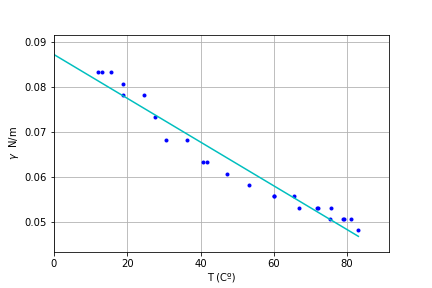
\includegraphics[width=11cm, height=7cm]{plot1-tensionsuperficial.png}
\caption{Representación de $\gamma$ frente a la temperatura del agua}
\label{fig:plot1-tensiónsuperfical}
\end{figure}

\newpage

\subsection{Estudio de la tensión superficial con diferentes disoluciones de alcohol} 
Una vez obtenemos los datos tenemos que:

\begin{table}[h!] %tabla de las disoluciones
\begin{center}
\begin{tabular}{|c|c|c|c|}
\hline
medida (i) & 	 \% etanol & 	 $F' \pm 0,001  \ (N)$ & 	 $\gamma \pm 0,025 \ (N/m) $ \\ \hline
1 & 	 10 & 	 0,092 & 	 0,0581 \\
2 & 	 20 & 	 0,088 & 	 0,0480 \\
3 & 	 30 & 	 0,086 & 	 0,0429 \\
4 & 	 40 & 	 0,084 & 	 0,0379 \\
5 & 	 50 & 	 0,082 & 	 0,0328 \\
6 & 	 60 & 	 0,082 & 	 0,0328 \\
7 & 	 70 & 	 0,081 & 	 0,0303 \\
8 & 	 80 & 	 0,080 & 	 0,0278 \\
9 & 	 90 & 	 0,080 & 	 0,0278 \\
10 & 	 100 & 	 0,079 & 	 0,0253 \\ \hline
\end{tabular}
\caption{valores de $\gamma$ para diferentes disoluciones de alcohol}

\label{tab:F' vs acetona}
\end{center}
\end{table}

Que representamos en la siguiente figura. Como podemos ver no hay una relación lineal $\gamma=a+b\cdot(\% \mathrm{alcohol})$, ya que traza una especie de curva. La curva azul que vemos es una aproximación hecha por python con un polinomio de grado dos, y podemos ver que en general los datos se aproximan bastante a esta curva. Por eso mismo no realizamos ningún tipo de regresión lineal en esta parte.

\begin{figure}[h!] %plot 2 tensión superficial
\centering
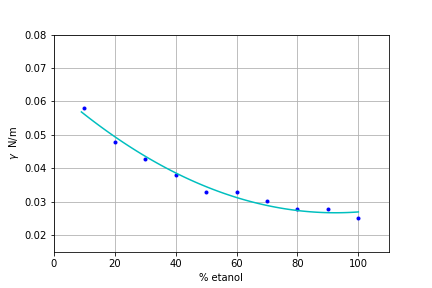
\includegraphics[width=11cm, height=7cm]{plot2-tensionsuperficial.png}
\caption{Representación de $\gamma$ frente al porcentaje de acetona en la disolución}
\label{fig:plot2-tensionsuperficial}
\end{figure}

\section{Conclusiones}
A lo largo de esta práctica hemos podido obtener los distintos valores del coeficiente de tensión superficial del agua para la temperatura ambiente, calcular cual es la relación temperatura-tensión y además ver como se comporta este valor en función del porcentaje de disolución del alcohol. Por lo tanto hemos cumplido todos los objetivos que nos marcamos al principio de la práctica. \\

Más allá de esto creo que hay varios puntos que debemos recalcar. En primer lugar, lo mas relevante es que la regresión lineal no es muy buena. Aunque el coeficiente de regresión lineal no este tan mal (0,97) si nos fijamos en el dibujo (en general) los datos van haciendo escalones, lo que hace que en general la regresión lineal no sea muy precisa. Esto se debe a que el dinamómetro que usamos tiene una precisión muy baja, y el indicador de la fuerza se queda postrado entre dos valores en bastantes ocasiones, lo cual dificulta bastante la toma de datos. Además muchas veces nos pasaba que el disco se iba hacia los lados de cristalizador, lo cual también hizo que tuviéramos que repetir medidas innecesariamente. Por otra parte también fue relevante haber usado hielo, ya que de otro modo la  temperatura habría bajado tan lentamente que tomar datos cercanos a 30 ºC hubiera sido eterno. Si quisiéramos mejorar la calidad de la práctica tendríamos que mejorar los aparatos. De todos modos los datos no están tan mal, con lo cual considero un éxito esta práctica, dadas las circunstancias. \\

Además pudimos aprender un fenómeno tan interesante que no habíamos visto hasta la fecha, y poder experimentar y estudiar como sucede es muy interesante, sobretodo por que la alta tensión superficial del agua es responsable de la vida, ayuda a mover el agua hasta la cima de los árboles, permite que la sangres se pegue a las paredes... 

%_______________________________MUELLE______________________________________



\chapter{Muelle}\label{Ch:muelle} \newpage


\section{Objetivos} \label{sec:muelle-objetivos}


En esta práctica trataremos de calcular la constante de equilibrio de un muelle de dos formas diferentes: una mediante el método estático, usando la ley de Hooke, y una mediante el método dinámico usando las ecuaciones del movimiento armónico simple. Además seremos capaces de calcular la densidad de un sólido y de un líquido. 

\section{Introducción teórica}


Como ya dijimos, vamos a tratar de calcular la contante de un muelle sujeto por su extremo a un soporte fijo del que cuelga una masa determinada \textbf{m}. Para esto tenemos dos métodos: el \textbf{método dinámico} y \textbf{método estático.} \\

El método dinámico se basa en la ley de Hooke, una ley que nos relaciona la fuerza que se ejerce sobre un muelle y cuanto se desplaza este de la posición de equilibrio:
\begin{equation}
F=-k \Delta x
\label{Ec: muelle ley de hooke}
\end{equation}
Esta fuerza será ejercida por una pesa, que se colgará en el extremo del muelle. Este ejercerá una fuerza denominada peso igual a:
\begin{equation}
F=P=g\cdot m
\label{Ec: muelle peso muelle}
\end{equation}
En nuestro caso no usaremos la g que sabemos todos (g=9,81$m/s^2$) si no la calculada en la siguiente práctica de caída libre, capítulo \ref{Ch: caída libre}. Esta será:
\begin{table}[h] %datos para calcular g
\begin{center}
\begin{tabular}{|c|c|}
\hline
$g \ (m/s^2)$ & 	 $s(g) \ (m/s^2)$  \\ \hline
9,335 & 	 0,067 \\  \hline
\end{tabular}
\label{Tab:caida libre-datos para calcular g - muelle}
\caption{valor de g y su incertidumbre}
\end{center}
\end{table}

De esta forma haremos una regresión lineal enfrentando a $F$ y $\Delta x$, de la cual obtendremos la pendiente ($b$), que será igual que nuestra k. 

\begin{equation}
k=b \label{Ec: muelle constante del muelle metodo estático}
\end{equation}

El método dinámico nos permite calcular la constante k a partir de el período de oscilación del muelle y la masa del objeto que pende. Si aplicamos las leyes de Newton al anterior ecuación obtenemos la ecuación de un movimiento armónico simple, del cual podemos extraer la siguiente ecuación, que relaciona el periódo angular del muelle con la masa que pende del objeto y su constante, de la siguiente forma:
$$ w=\sqrt{\dfrac{m}{k}}$$
Trasformando el periodo angular en el periodo:
\begin{equation}
T=2\pi \sqrt{\dfrac{m}{k}}
\label{Ec: muelle período realcionado con k muelle}
\end{equation}
Y elevando todo al cuadrado:
\begin{equation}
T^2=4 \pi^2 \dfrac{m}{k}
\label{Ec: muelle periodo al cuadrado relacionado con k muelle}
\end{equation}
De esta forma podemos construir una regresión lineal que enfrente el periodo al cuadrado y el producto de la masa por $4\pi$ tal que:
$$ T^2=b 4\pi m$$
De lo cual podemos extraer que:
\begin{equation}
b=\dfrac{1}{k}
\label{Ec: muelle b realacionado con k muelle}
\end{equation}
De aquí podemos extraer la constante del muelle y su incertidumbre. \\

Ahora viene la parte en la que calculamos la densidad del un sólido a partir de la densidad de un líquido, que podemos calcularlo conociendo la distancia del objeto ($\Delta x$) a la posición en el aire y conociendo esta misma distancia pero con el objeto sumergido en el líquido ($\Delta x'$). Como el líquido ejerce una fuerza de flotación sobre el sólido, igual a la densidad del líquido por el volumen desplazado y g, con sentido opuesto a la fuerza que ejerce el peso; y tenemos que $\Delta x'$ será menor que $\Delta x$ por esto mismo (debido a que la fuerza neta es menor cuando existe fuerza de flotación), podemos deducir que:
\begin{equation}
\rho_s=\rho_L \cdot \dfrac{\Delta x}{\Delta x - \Delta x'}
\label{Ec: muelle densidad del sólido muelle}
\end{equation}
En la primera parte calcularemos la densidad de diferentes sólidos usando el agua como líquido, del cual asumiremos que $\rho_{agua}=1 g/mL$. Una vez calculados estos podremos despejar la densidad del líquido y obtener la densidad de un líquido a partir de la densidad del sólido. De esta forma calcularemos la densidad de la cetona.
\begin{equation}
\rho_L=\rho_s \cdot \dfrac{\Delta x - \Delta x'}{\Delta x}
\label{Ec: muelle densidad del líquido muelle}
\end{equation}

\section{Montaje experimental}
\subsection{Calculo de k}
En la primera parte de esta práctica calculamos la constante k de un muelle. Como ya dijimos existen dos métodos. En el \textbf{estático} primero medimos la distancia entre extremo y extremo del muelle sin ningún tipo de masa colgando. Esto se hará con un \textbf{soporte} lo suficientemente alto como para colgar el muelle sin que toque la mesa de trabajo o el suelo. La distancia la mediremos con una \textbf{regla} de precisión milimétrica, por eso la precisión de $x_0$ y $x$ será de 1mm. Una vez calculamos con la regla la posición del extremo inferior del muelle, cogemos las diferentes masas, las cuales medimos con una \textbf{balanza} de precisión $0,01 \ g$, por lo que será nuestra incertidumbre , y las colgamos de dicho extremo. Debido a la masa que ejerce una fuerza (el peso) sobre el muelle este se estirará. Ahora medimos la posición del extremo del muelle, y calculamos la diferencia:
\begin{equation}
\Delta x = x_0-x
\label{Ec: muelle diferencia de x}
\end{equation}
Como se puede ilustrar en la figura siguiente la $\Delta x$ que calculamos es la distancia entre las bandas rojas inferiores. De esta forma tendremos todos los datos necesarios para calcular la fuerza, y representarlo frente a esta distancia.  \\

\begin{figure}[h!]
\centering
\begin{subfigure}[b]{0.3\linewidth}
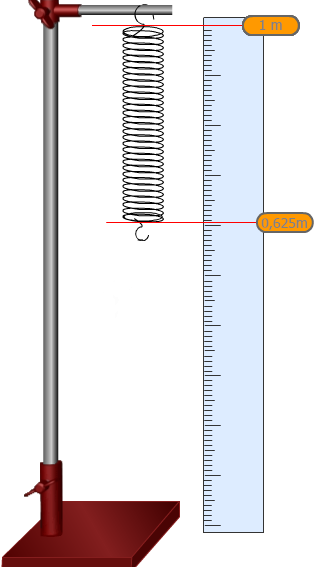
\includegraphics[scale=0.35]{muelle-dibujo1.png}
\caption{muelle sin peso}
\label{fig: muelle sin peso}
\end{subfigure}
\begin{subfigure}[b]{0.3\linewidth}
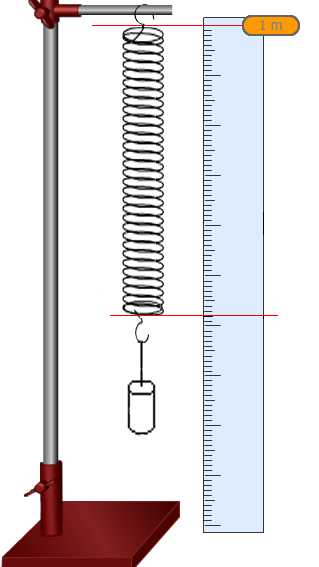
\includegraphics[scale=0.35]{muelle-dibujo2.png}
\caption{muelle con peso}
\label{fig: muelle con peso}
\end{subfigure}
\label{fig: muelle figura}
\caption{muelle con y sin peso}
\end{figure}

Para calcular k mediante el \textbf{método dinámico} debemos de conocer tanto el periodo de oscilación del muelle y la masa que cuelga del mismo. Para calcular la masa usamos el mismo método que antes: una \textbf{balanza}, con la misma precisión (0,01 $g$). Entonces solo nos queda por conocer el periodo de oscilación. Este se puede calcular simplemente ejerciendo una fuerza hacia abajo en el muelle, y calcular el tiempo en que tarda en regresar. Sin embargo este método de calcular T sería muy poco preciso, ya que aunque la precisión del \textbf{cronómetro} que vamos a usar es de 0,01 $s$, debido al tiempo de reacción del ser humano (entorno a 0,3 segundos) la incertidumbre es mucho mas grande. Para tratar de reducirla  lo que hacemos es medir cuanto tarda en regresar 10 veces al punto de partida. Es decir, medimos 10T, 10 veces el periodo, y como la precisión de 10T será de 0,3 $s$; habremos reducido a un 10\% la incertidumbre del periodo. Ahora ya tendríamos todos datos necesarios para calcular la constante k por este método.

\subsection{Calculo de densidades}

Para calcular la densidades con el muelle lo que haremos es emplear la estática de fluidos, como hemos mencionado anteriormente. Como primero nos piden calcular la densidad de 3 sólidos, entonces lo que haremos será usar un líquido cuya densidad conozcamos, como el agua. Entonces rellenaremos un vaso de precipitación de agua y la colocaremos en una plataforma que nos ayudará a subir el vaso y mantenerlo fijo. Entonces iremos subiendo la plataforma hasta que el sólido se sumerja por completo.\\

En este momento anotaremos la $\Delta x'$. Como previamente (o posteriormente) hemos calculado la $\Delta x$ (sin sumergir) del sólido ya podremos calcular la densidad del mismo. \\

Ahora tendremos que calcular la densidad de un líquido no conocido. Pero como conocemos las densidades de los sólidos podremos calcular perfectamente la densidad del líquido, invirtiendo la fórmula \ref{Ec: muelle densidad del líquido muelle}. El único procedimiento que tendremos que hacer aquí será sumergir de nuevo las pesas pero en la cetona.


\section{Análisis de datos}

\subsection{Determinación de k por el medio estático}
En esta parte primero obtendremos el valor de las masas y del estiramiento del muelle con las masas, para luego realizar la regresión lineal. El estiramiento asociado a una masa cualquiera m vendrá dada por la ecuación \ref{Ec: muelle diferencia de x}, por lo que la incertidumbre de dicho estiramiento es:

\begin{equation}
s(\Delta x)=\sqrt{[s(x_0)]^2+[s(x)]^2}
\end{equation}
Que como ambas incertidumbres son 1mm, tenemos que $s(\Delta x)=1,4mm$.  \\

Ahora debemos calcular la fuerza que se ejerce, que podemos calcular facilmente sabiendo las masas usando la ecuación \ref{Ec: muelle peso muelle}. La incertidumbre asociada a dicha fuerza será:

\begin{equation}
s(F)=\sqrt{g^2s^2(m)+m^2s(g)}
\label{Ec: muelle incertidumbre F}
\end{equation}

Ahora representamos el estiramiento asociado a cada masa, así como la fuerza a la que equivale dicha masa y su incertidumbre: 
 
\begin{table}[h!] %datos de f vs delta x
\begin{center}
\begin{tabular}{|c|c|c|c|}
\hline$ m \pm 0,01 \ (g) $ & 	 $ \Delta x \pm 1,4 \ (mm) $ & 	 $F \ (mN) $ & 	 $s(F) \ (mN)$ \\ \hline
60,56 & 	 196 & 	 566,5 & 	 4,1 \\ 
70,78 & 	 226 & 	 662,1 & 	 4,7 \\ 
80,53 & 	 259 & 	 753,4 & 	 5,4 \\ 
100,52 & 	 324 & 	 940,4 & 	 6,7 \\ 
109,94 & 	 352 & 	 1028,5 & 	 7,4 \\ 
120,48 & 	 386 & 	 1127,1 & 	 8,1 \\ 
129,90 & 	 416 & 	 1215,2 & 	 8,7 \\ 
140,43 & 	 450 & 	 1313,7 & 	 9,4 \\ 
149,86 & 	 480 & 	 1402 & 	 10 \\ 
159,76 & 	 510 & 	 1494 & 	 11 \\ \hline
\end{tabular}
\label{Tab:Muelle delta x vs F}

\caption{datos sobre la fuerza ejercida sobre un muelle y su estiramiento}
\end{center}
\end{table}

Una vez tenemos todos estos datos ya estamos preparados para realizar la regresión lineal. Sin embargo, aquí se nos plantea una duda: ¿Que tipo de regresión lineal usamos?. Como podemos ver la incertidumbre de los datos va cambiando, por lo que deberíamos hacer una regresión lineal ponderada. Sin embargo, dado que la variación de s(F) es muy pequeña (no llega ni a un orden de diferencia entre la incertidumbre mas pequeña y la más grande) y que la incertidumbre de $\Delta x$ es mas pequeña realizaremos la regresión lineal simple. Además será sin termino independiente, ya que la ley de hooke que usamos para obtener k no tiene ningún término independiente. Los valores que obtenemos son los representados en la tabla \ref{Tab:muelle-valor de k, s(k) y r} (ponemos k ya que b=k, y s(b)=s(k)) \\

\begin{table}[h] %datos de k, s(k) y r
\begin{center}
\begin{tabular}{|c|c|c|}
\hline
$k \ (N/m) $ & 	 $s(k) \ (N/m) $ & 	 r \\ \hline
2,9200 & 	 0,0029 & 	 0,999995 \\ 
\hline
\end{tabular}
\caption{valor de k, su incertidumbre y el coeficiente de regresión lineal}
\label{Tab:muelle-valor de k, s(k) y r}
\end{center}
\end{table}

Como podemos observar la regresión lineal es muy precisa, ya que r nos da con 6 cifras, lo cual es un indicativo de lo buena que es la regresión. A pesar de que deberíamos haberla hecha ponderada dicho resultado nos reafirma que en realidad podemos aproximar la regresión lineal por una simple, representada en la figura siguiente. 

\begin{figure}[h!] %plot 1 muelle
\centering
\includegraphics[width=11cm, height=7cm]{Plot1-muelle.png}
\caption{Representación de $F$ vs $\Delta x$ }
\label{fig:Plot1-muelle}
\end{figure}

\subsection{Determinación de k por el medio dinámico}
En esta parte calcularemos k usando la ecuación \ref{Ec: muelle periodo al cuadrado relacionado con k muelle}. Para esto tendremos que calcular el periodo al cuadrado asociado a $4 \pi^2 m$, así como la incertidumbre asociadas a estos valores, que vienen dadas por las ecuaciones: 

\begin{equation}
s(T^2)=\sqrt{(2T)s^2(T)}=2Ts(T)
\label{Ec: muelle incertidumbre del periodo muelle}
\end{equation}

\begin{equation}
s(4\pi^2m)=\sqrt{(4\pi^2)^2s^2(m)}=4 \pi^2 s(m)
\label{Ec: muelle incertidumbre de 4pim muelle}
\end{equation}

Como ya hemos dicho, para calcular T lo que hacemos es obtener 10T y luego dividir 10T entre 10. Como es evidente, la incertidumbre de T también variará, por lo que haciendo propagación de incertidumbres:
\begin{equation}
s(T)=\sqrt{\dfrac{[s(10T)]^2}{10^2}}=\dfrac{s(10T)}{10}
\end{equation}
Y como s(10T)=0,3 s (tiempo de reacción del ser humano) obtenemos que s(T)=0,03 s. Además como la masa la medimos en gramos pero queremos la constante en unidades del SI tendremos que convertirlo a kg teniendo en cuenta que 1kg=1000g. Mediante propagación de incertidumbres calculamos la nueva incertidumbre asocaida (llamando $m_0$ a la masa en gramos):
\begin{equation}
s(m)=\sqrt{s(m_0)\cdot 0,001^2}=s(m_0)\cdot 0,001
\end{equation}
Una vez tenemos todos estos datos, representamos en la tabla \ref{Tab:muelle-valor de T y m} todos ellos, con el periodo asociado a cada masa, así como el periodo al cuadrado y $4 \pi^2 m$, que son al final los datos que usaremos para calcular la regresión lineal. \\

\begin{table}[h!] %datos de T, m, 4pim...
\begin{center}
\begin{tabular}{|c|c|c|c|c|}
\hline

$ m \pm 0,00001 \ (Kg) $ & 	 $T \pm 0,03 \ (s) $ & 	 $ 4\pi^2 m \pm 0,00039 \ (Kg) $ & 	 $T^2 \ (s) $ & 	 $s(T^2) \ (s)$
 	\\ \hline
0,06056 & 	 0,92 & 	 2,39081 & 	 0,845 & 	 0,055
 	\\
0,07078 & 	 1,01 & 	 2,79428 & 	 1,026 & 	 0,061
 	\\
0,08053 & 	 1,06 & 	 3,17920 & 	 1,130 & 	 0,064
 	\\
0,10052 & 	 1,16 & 	 3,96837 & 	 1,353 & 	 0,070
 	\\
0,10994 & 	 1,24 & 	 4,34026 & 	 1,525 & 	 0,074
 	\\
0,12048 & 	 1,28 & 	 4,75636 & 	 1,641 & 	 0,077
 	\\
0,1299 & 	 1,33 & 	 5,12825 & 	 1,764 & 	 0,080
 	\\
0,14043 & 	 1,38 & 	 5,54395 & 	 1,891 & 	 0,083
 	\\
0,14986 & 	 1,43 & 	 5,91624 & 	 2,031 & 	 0,086
 	\\
0,15976 & 	 1,47 & 	 6,30707 & 	 2,155 & 	 0,088
 	\\
\hline
\end{tabular}
\caption{datos necesarios para calcular k por medio dinámico}
\label{Tab:muelle-valor de T y m}
\end{center}
\end{table}

Ahora, de nuevo, se nos presenta la duda de que tipo de regresión lineal hacer, ¿Simple o ponderada? Al igual que antes, la variación de la incertidumbre de $T^2$ es casi despreciable, y como s(m)$<$s($T^2$) podremos hacer una regresión lineal simple sin término independiente, ya que en la fórmula que usamos para calcular k (ecuación \ref{Ec: muelle periodo al cuadrado relacionado con k muelle}) no aparece ningún término independiente. De esta forma podremos obtener la pendiente, su incertidumbre y el coeficiente de regresión lineal asociado, representados en la tabla \ref{Tab:muelle-valor de b, s(b) y r}.  \\ 

\begin{table}[h!] %datos de b, s(b) y r
\begin{center}
\begin{tabular}{|c|c|c|}
\hline
$ b  \ (m/mN) $ & 	 $s(b)  \ (m/mN) $ & 	 r \\  \hline
0,3452 & 	 0,0020 & 	 0,9998 \\ 
\hline
\end{tabular}
\caption{valor de b, s(b) y el coeficiente de regresión lineal}
\label{Tab:muelle-valor de b, s(b) y r}
\end{center}
\end{table}

Al igual que antes podemos ver que a pesar de aproximar por una regresión lineal simple (que representamos gráficamente en la imagen \ref{fig:Plot2-muelle}) el coeficiente de regresión lineal nos da un valor bastante cercano a 1: la regresión lineal está bien hecha. \\

Una vez tenemos b, ya podemos calcular k y s(k) teniendo en cuenta la ecuación \ref{Ec: muelle b realacionado con k muelle}. y que  haciendo propagación de incertidumbre la incertidumbre vendrá dada por:

\begin{equation}
s(k)=\sqrt{(\dfrac{1}{b^2})^2[s(b)]^2}=\dfrac{1}{b^2}s(b)
\label{EC: muelle incertidumbre de k por el periodo muelle}
\end{equation}

\begin{table}[h!] %datos de k, s(k)
\begin{center}
\begin{tabular}{|c|c|}
\hline
$ k \ (N/m)$ & 	 $s(k) \ (N/m)$ \\ \hline
2,897 & 	 0,017 \\
\hline
\end{tabular}
\label{Tab:muelle-valor de k, s(k)}
\caption{valor de k y su incertidumbre}
\end{center}
\end{table}

\begin{figure}[h!] %plot 2 muelle
\centering
\includegraphics[width=11cm, height=7cm]{Plot2-muelle.png}
\caption{Representación de $T^2$ (T = periodo) vs $4 \pi m$ (m = masa)}
\label{fig:Plot2-muelle}
\end{figure}


\subsection{Cálculo de la densidad de un sólido}

En esta parte calculamos la densidad del sólido mediante la fórmula \ref{Ec: muelle densidad del sólido muelle}. Entonces para cada pesa debemos calcular el estiramiento en el aire y el estiramiento cuando están sumergidos en el agua. Además tenemos que tener en cuenta la incertidumbre de la densidad, que verificará la siguiente fórmula: 

\begin{equation}
s(\rho_s)=\sqrt{s^2(\Delta x) (\dfrac{\Delta x'}{(\Delta x - \Delta x')})^2+s^2(\Delta x')(\dfrac{\Delta x}{(\Delta x - \Delta x')^2})^2}
\label{Ec: muelle densidad del sólido muelle incertidumbre}
\end{equation}

En la siguiente tabla podemos observar los datos para cada pesa, junto con su densidad e incertidumbre:

\begin{table}[h!] %datos de k, s(k)
\begin{center}
\begin{tabular}{|c|c|c|c|c|}
\hline
Medida & 	 $\Delta x \pm 1,4 \ (mm) $ & 	 $\Delta x'_{agua} \pm 1,4 \ (mm) $ & 	 $\rho_{solido} \ (g/mL) $ & 	 $s(\rho) \ (g/mL) $
  	\\ \hline 
Solido 1 (aluminio) & 	 155 & 	 99 & 	 2,760 & 	 0,082
  	\\ 
Solido 2 & 	 389 & 	 331 & 	 6,7 & 	 0,21
  	\\ 
Solido 3 & 	 234 & 	 203 & 	 7,5 & 	 0,45
 	\\  \hline
\end{tabular}
\caption{valor de $\rho$ para diferentes metales y su incertidumbre}
\label{Tab:muelle-valor de la densidad de metales}
\end{center}
\end{table}

Aunque ya lo comentaremos con profundidad mas adelante, podemos observar que las las incertidumbres son realmente altas, debido a que hay que tener en cuenta muchos datos e incertidumbres en la fórmula. Además podemos observar que la densidad del sólido 1 es muy próxima a la del aluminio (2,7 g/mL), de hecho, si nos fijamos $2,7 \in (2,760-0,082 \ ; \ 2,760+0,082) $, es decir, está en el margen de la incertidumbre, por lo que podemos concluir que el sólido 1 es aluminio.

\subsection{Cálculo de la densidad de un líquido}
En esta parte calcularemos la densidad de la cetona. Para esto tenemos los datos de las densidad de los sólidos que vamos a utilizar y sus incertidumbres (véase tabla \ref{Tab:muelle-valor de la densidad de metales}). Entonces como sabemos que la densidad de un líquido viene dada por la ecuación \ref{Ec: muelle densidad del líquido muelle}, realizando propagación de incertidumbres podemos saber que la incertidumbre se calcula con la siguiente ecuación:

\vspace*{0.2cm}

\begin{equation}
s(\rho_s)=\sqrt{s^2(\Delta x)\rho_s^2(\dfrac{\Delta x'}{x})^2+s^2(\Delta x')\rho_s^2(\dfrac{1}{\Delta x})^2+s^2(\rho_s)(\dfrac{\Delta x - \Delta x'}{\Delta x})^2}
\label{Ec: muelle densidad del líquido muelle incertidumbre}
\end{equation}

\vspace*{0.2cm}

Ahora teniendo en cuenta toda esta información, volvemos a sumergir las pesas de la cual extraemos un $\Delta x'$ nuevo, y podemos obtener la densidad de la cetona, representada en la siguiente tabla:

\begin{table}[h!] %datos de k, s(k)
\begin{center}
\begin{tabular}{|c|c|c|c|c|}
\hline
Medida & 	 $\Delta x \pm 1,4 \ (mm) $ & 	 $\Delta x'_{cetona} \pm 1,4 (mm) $ & 	 $\rho_{cetona} \ (g/L) $ & 	 $s(\rho) \ (g/mL) $
  	\\ \hline
Solido 1 (aluminio) & 	 155 & 	 110 & 	 0,801 & 	 0,039
  	\\ 
Solido 2 & 	 389 & 	 344 & 	 0,774 & 	 0,040
  	\\ 
Solido 3 & 	 234 & 	 211 & 	 0,740 & 	 0,075  	\\   \hline
\end{tabular}
\caption{valor de $\rho$ para la cetona y su incertidumbre a partir de diferentes sólidos}
\label{Tab:muelle-valor-densidad-liquidos}
\end{center}
\end{table}

Al igual que antes, la incertidumbre es muy grande, pero esto se debe a que no solo tenemos en cuenta la incertidumbre de los estiramientos, si no que también tenemos en cuenta la de las densidades de los sólidos, que ya de por si son bastante altas, sobretodo en el tercer sólido que solo con su incertidumbre abarca las otras dos densidades. Ahora realizaremos una media (y la incertidumbre de esta) para ver el valor final que nos quedaría la densidad de la cetona. Como tenemos diferente medidas de la misma magnitud, con diferentes incertidumbres usaremos fórmulas diferentes a las citadas en el capítulo 1, ya que usaremos las fórmulas de la media ponderada, que tiene en cuenta las incertidumbres de los cálculos. Como realmente tiene poco interés citar las fórmulas, simplemente realizaremos los cálculos, de los cuales obtenemos que:

\begin{table}[h!]
\centering
\begin{tabular}{|c|c|}
\hline
$\rho_{cetona} $ & $s(\rho_{cetona})$ \\ \hline
0,782 & 0,026 \\ \hline
\end{tabular}
\caption{media ponderada de $\rho_{cetona}$ e incertidumbre}
\label{Tab:muelle-densidad-cetona}
\end{table}

Que como podemos observar es un valor relativamente similar al de la cetona (0,782 g/L). De hecho este valor está dentro de la incertidumbre del que nosotros obtuvimos.

\section{Conclusiones}
Una vez tenemos todos los datos calculados, veamos, en primer lugar si hemos cumplido los objetivos que nos habíamos propuesto al principio. Luego podremos discutir otros puntos relevantes, tales como problemas, diferencias entre incertidumbres... \\

Los dos objetivos principales que nos pusimos al empezar la práctica (véase sección \ref{sec:muelle-objetivos}) fueron calcular la constante k del muelle y la densidad de unos sólidos y de la cetona. Podemos observar que la parte de calcular la constante k del muelle fue todo un éxito, ya que comparando los dos valores de las constantes:

\begin{table}[h!]
\centering
\begin{tabular}{|c|c|}
\hline
$k_1$ (N/m) & $k_2$  (N/m) \\ \hline
2,9200 $\pm$ 0,0029 & 2,897 $\pm$ 0,017 \\ \hline
\end{tabular}
\caption{valores de k}
\end{table}

Ambos valores son realmente similares. Esto también ya se podía observar cuando los coeficientes de regresión lineal nos dieron valores tan próximos a 1. Sin embargo podemos ver que $k_2$, es decir, la constante calculada por el método dinámico tiene una incertidumbre mas grande que $k_1$. Esto se debe principalmente a que los datos tomados para calcular ($T^2$...) son más difíciles de cuantificar que simplemente un estiramiento (como en $k_1$), por lo que la incertidumbre es mayor, y esta al final se acaba propagando. Aun así sigue siendo una incertidumbre ridícula, en comparación con el dato, sobretodo cuando veamos las incertidumbres de las densidades, muchísimo mas altas en proporción a los datos. \\

Ahora bien, ¿Que podemos concluír de esta parte de la práctica? Pues analizando todo, principalmente dos cosas: personalmente la que me parece mas impactante es que realmente la ley de hooke y el movimiento armónico simple de un muelle realmente tienen una relación directa, no solo teóricamente, si no experimentalmente: nos ha dado prácticamente la misma constante. Y aunque hemos supuesto que era un muelle ideal, no lo era, y a pesar de todo estas dos fórmulas han dado valores idénticos. La otra conclusión que podemos extraer es que se verifica la ley de hooke para un muelle, ya que en función de la fuerza que ejercemos se estirara mas o menos el muelle, con una relación lineal directa, tal y como podemos observar en la figura \ref{fig:Plot1-muelle}. \\

La otra parte de la práctica nos pedía calcular la densidad de unos sólidos, y luego a partir de los datos obtenidos obtener la densidad de la cetona. En las tablas \ref{Tab:muelle-valor de la densidad de metales} y \ref{Tab:muelle-densidad-cetona}, dicho objetivo está cumplido. De hecho podemos ver que el sólido 1 tiene una densidad próxima a la del aluminio: $2,760 \footnote{desnidad aluminio experimental} \approx 2,7 \footnote{densidad aluminio}$; y que la cetona también tiene un valor cercano al real; $0,782 \footnote{densidad cetona experimental} \approx 0,784 \footnote{densidad cetona}$; por lo que podemos concluir que está bien hecho. Aún con todo no son cifras escandalosamente parecidas. Es mas, de no ser porque los valores reales se encuentran dentro de las incertidumbres, hasta podríamos dudar de la calidad del experimento. Sin embargo, ¿Por qué podemos decir que el experimente está bien hecho?. Y yendo un poco mas allá, ¿Por qué las incertidumbres son tan grandes?. Ambas respuestas se solapan, ya que podemos a la primera pregunta podríamos argumentar que los datos reales están dentro de las incertidumbres, pero realmente es que las incertidumbes tienen valores bastante altos, como en el caso de la cetona calculada con el sólido 3, que es mas de un 10\% el error realtivo. La razón de esta proporción se encuentra en la propia naturaleza del experimento: al realizar una sóla medida, la probabilidad de que salga un valor no real es bastante grande, y mas si para calcular los valores de las diferentes densidades tenemos en cuenta tantos datos, ya que se acumularán los errores. Por esa razón, aunque en realidad no den datos tan parecidos como las constantes, lo parecidos que son es un buen indicativo, ya que a pesar de haber realizado una sola medida, si que se parecen (sobretodo con la cetona). \\

Al igual que antes nos preguntamos que podemos extraer de esta parte de la práctica, mi respuesta sería que hemos aprendido un buen método para calcular densidades de sólidos y líquidos, bastante sencilla de hacer (ya que solo hace falta un soporte y un muelle), y que podría tener muchas utilidades, sobretodo para la física mas aplicada y las ingenierías.


 
 


%_________________CAIDA LIBRE_____________




\chapter{Caída libre }\label{Ch: caída libre} \newpage
\section{Objetivos}
El objetivo de esta práctica es calcular la constante de la gravedad, para utilizar dicho valor obtenido en la práctica de muelle (capitulo \ref{Ch:muelle}).
\section{Introducción teórica}
En este caso calcularemos la aceleración de la gravedad a partir de la fórmula de caída libre. Esta fórmula nos dice que:

\begin{equation}
d=\dfrac{1}{2}gt^2
\label{Ec: ecuación del movimiento caida libre}
\end{equation}

Que podemos reescribirla como: 


\begin{equation}
t^2g=2d
\label{Ec: ecuación que relaciona g con t y d caida libre}
\end{equation}


Siendo d la distancia que recorre el objeto que hasta que el objeto deja de caer, y t el tiempo que tarda el objeto en caer. Ahora para calcular g lo que haremos es una regresión lineal que enfrente 2d y $t^2$, y de esta forma el valor de la pendiente será el mismo de g, por lo que:
$$ b = g, \ \ s(b) = s(g) $$
Sin embargo, tendremos que calcular las incertidumbres tanto de s(2d) y de s($t^2$), para así saber que tipo de regresión lineal hacer. Dichas incertidumbres vienen dadas por: \\

\begin{equation}
s(t^2)=\sqrt{s^2(t)(2t)^2}=2ts(t)
\label{Ec: t^2 incertidumbre caida libre}
\end{equation}

\begin{equation}
s(2d)=\sqrt{s^2(d)2^2}=2S(d)
\label{Ec: 2d incertidumbre caida libre}
\end{equation}

Dicho esto, ya tenemos todas las fórmulas y teoría necesaria para calcular la constante g.

\section{Montaje experimental}
Para calcular d y t usaremos un aparato del cual dejamos caer una bola de metal, y que gracias a un imán nos ayuda a mantenerlo sujeto. Cuando pulsamos un botón el propio aparato deja caer la bola, y además inicia un cronómetro que una vez que llega al final del objeto se para automáticamente. La dificultad de este proceso es medir la distancia d, ya que se hace con una regla, lo cual dificulta mucho la medida. Además la bola también hace más difícil esta medida, ya que tenemos que tener en cuenta su diámetro. Por todas estas razones la incertidumbre de d es de 0,3 cm. La incertidumbre de t es de 0,01 ms ya que es la precisión del aparato.

\section{Análisis de datos}

Una vez obtenemos los calculamos la altura, podemos soltar la bola y calcular t. Una vez tenemos los datos, calculamos $t^2$ y $2d$. Representando los datos en la tabla:

\begin{table}[h] %datos para calcular g
\begin{center}
\begin{tabular}{|c|c|c|c|c|}
\hline
$d  \pm 0,3 \ \ (cm)$ & 	 $t \pm 0,01 \ \ (ms)$ & 	 $2d  \pm 0,6 \ \ (m)$ & 	 $t^2  \ \ (s)$ & 	 $s(t^2) \ \ (s)$
 	\\ \hline
56,5 & 	 345,07 & 	 1,13 & 	 0,1190733 & 	 0,0000024
 	\\
52,5 & 	 339,00 & 	 1,05 & 	 0,1149210 & 	 0,0000023
 	\\
48,7 & 	 319,13 & 	 0,974 & 	 0,1018440 & 	 0,0000020
 	\\
44,9 & 	 313,80 & 	 0,898 & 	 0,0984704 & 	 0,0000020
 	\\
40,8 & 	 299,57 & 	 0,816 & 	 0,0897422 & 	 0,0000018
 	\\
38,7 & 	 286,65 & 	 0,774 & 	 0,0821682 & 	 0,0000016
 	\\
33,7 & 	 266,81 & 	 0,674 & 	 0,0711876 & 	 0,0000014
 	\\
30,7 & 	 256,13 & 	 0,614 & 	 0,0656026 & 	 0,0000013
 	\\
26,5 & 	 239,93 & 	 0,53 & 	 0,0575664 & 	 0,0000012
 	\\
22,5 & 	 213,32 & 	 0,45 & 	 0,04550542 & 	 0,00000091
 	\\ \hline
\end{tabular}
 \label{Tab:caida libre-datos para calcular g}
\caption{datos para calcular g}
\end{center}
\end{table}

Una vez tenemos estos datos ya podemos hacer una regresión lineal, ahora bien, cual hacemos. Como podemos ver, la incertidumbre de 2d es muchísimo mas grande que la de $t^2$. A pesar de que esta varíe, por ser despreciable frente a s(d) podemos hacer una regresión lineal simple. Una vez hecha tenemos que los valores de g y s(g) (b, s(b)) y el coeficiente de regresión lineal son:

\begin{table}[h] %datos para calcular g
\begin{center}
\begin{tabular}{|c|c|c|}
\hline
$g \ (m/s^2)$ & 	 $s(g) \ (m/s^2)$ & 	 r \\ \hline
9,335 & 	 0,067 & 	 0,9997 \\  \hline
\end{tabular}
\label{Tab:caida libre-datos para calcular g}
\caption{valor de g y su incertidumbre}
\end{center}
\end{table}

Como podemos ver r tiene un valor muy cercano a 1, lo cual está muy bien. Representando gráficamente dichos valores: 



\begin{figure}[h!] %caida libre plot 1
\centering
\includegraphics[width=11cm, height=7cm]{Plot1-caidalibre.png}
\caption{Representación de $2d$ vs $t^2$ (t=tiempo)}
\label{fig:Plot1-caidalibre}
\end{figure}


\section{Conclusiones}
En este caso hemos calculado g a partir de el tiempo y distancia de caida de una bola. Como sabemos todos, el valor de g=9,81 m/$s^2$. Como se puede ver hay una notable diferencia entre este valor y el obtenido, ya que ni siquiera esta en el rango de incertidumbre de la medida. Las razones por las que sucede esto se deben a la elevada dificultad de medir la altura, ya que usamos aparatos muy poco precisos, difíciles de colocar bien y bastante rudimentarios. Sería necesario una mejora del los instrumentos para obtener un valor mas próximo al real. Aun con todo si que tienen cierto parecido, por lo que tampoco podemos descartar dicho dato. Para tratar de mejorar la muestra también podríamos realizar mas medidas, ya que 10 puede que sean pocas. 


%________________________________KATER______________________________________



\chapter{Kater} \newpage

\section{Objetivos}
El objetivo de esta práctica es determinar la aceleración de la gravedad g mediante la utilización de un péndulo kater.
\section{Introducción teórica}
Un péndulo es un cuerpo sólido que puede oscilar libremente en el espacio respecto a un eje (horirzontal en nuestro caso) gracias a una fuerza (la gravitatoria), que se traduce en dos fuerzas: una es el par generado por su pes, aplicado en el cetro de gravedad del cuerpo, y la fuerza de reacción del eje fijo, aplicada en el punto de suspensión. Entonces si separamos el péndulo de la posición de equilibrio este comenzara a oscilar adquiriendo un movimiento armónico simple (MAS) que viene dado por:
\begin{equation}
T=2\pi \sqrt{\dfrac{I}{m \ g \ h}}
\label{Ec:kater-periodo-momento-incercia}
\end{equation}
Como sabemos por el teorema de Steiner el momento de inercia respecto a un eje cualquiera del péndulo será igual al momento de incercia sobre el centro de gravedad G del péndulo sumado al producto de la masa por el cuadrado de la distancia que separa dichos dos ejes, es decir:
\begin{equation}
I=I_G+mh^2
\label{Ec:kater-teorema-steiner}
\end{equation}

Entonces sustituyendo dicha ecuación en la ecuación \ref{Ec:kater-periodo-momento-incercia}, y elevando al cuadrado ambos lados, tenemos que:
\begin{equation}
\dfrac{T^2}{4 \pi^2}=\dfrac{I_G+mh^2}{m \ g \ h}
\label{Ec:kater-periodo2-momento-incercia}
\end{equation}
Como podemos ver conociendo tanto la masa, el periodo y la distancia del eje al centro de masas podríamos obtener g, excepto porque aparece el momento de inercia. Sin embargo, si fuéramos capaces de despejar este, tendríamos la capacidad para obtener los otros datos, y obtener el valor de g. Esto lo veremos en el siguiente capítulo.

\section{Montaje experimental}
Como ya hemos adelantado, tenemos que ser capaces de despejar de algún modo $I_G$, y luego obtener los demás datos. Para esto aprovecharemos las características del péndulo kater. El péndulo kater está formado por una barra metálica con dos cuchillas al final de la barra ($E_1$ y $E_2$), y dos masas móviles, una a cada lado del péndulo (C y D), ya que este está partido en dos mitades, como se puede ver en la imagen \ref{Fig:kater-pendulo} \\

\begin{figure}
\centering
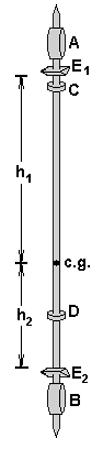
\includegraphics[scale=0.5]{kater-dibujo1.png}
\caption{pendulo kater}
\label{Fig:kater-pendulo}
\end{figure}

En función de las posiciones de las masas el centro de masas G (c.g. en la figura). Para saber el punto exacto del centro de masas nos ayudaremos de un \textbf{soporte} en el cual tiene en el centro un punto de apoyo donde podemos colocar el péndulo, y si ese punto de apoyo coincide con el centro de gravedad, el péndulo estará en equilibrio. Si en dicho punto de apoyo no colocamos el centro de gravedad, el péndulo no estará en equilibrio y se irá hacia uno de los lados. Es un comportamiento similar al de un balancín. Ahora podremos saber la posición de G, y por lo tanto medir la distancia $h_1$ que será la distancia desde G hasta $E_1$, y $h_2$, que será la distancia desde G hasta $E_2$; con la misma distribución de masas, sin cambiar la posición de las pesas. Como usamos un \textbf{metro} para medir la distancia entre el centro de masas y las masas, cuya precisión es de 0,001 metros. Sin embargo debido a la dificultad para mantener la cinta el metro recta y otros problemas asociados (dificultad de ver cual es el punto exacto de G...) nosotros decidimos poner la incertidumbre en 0,002 m, aunque podría ser más. \\

Una vez tenemos claro esto, podemos pender el péndulo por el $E_1$, de tal modo que lo dejamos oscilar libremente y calculamos el periodo colocado en este eje, eje el cual su momento de incercia será $I_G + mh_1^2$, del cual conocemos solo $h_1$. Para reducir la incertidumbre de la medida medimos  el tiempo en que tarda oscilar 5 periodos, aunque si quisiéramos reducir mas este valor podríamos llegar hasta 10. Nosotros realizamos 5 debido a un fallo de cálculo, del cual posteriormente nos dimos cuenta. De esta forma obtendríamos dicho periodo:
\begin{equation}
T_1=\dfrac{t_1}{5}
\label{Ec: kater valor del periodo 1 kater}
\end{equation}
Así obtendríamos una incertidumbre mucho menor, ya que en este caso no es la inceritumbre del cronómetro (entorno a 0,01s) si no que sería nuestra capacidad de reacción, que es de 0,3s. Si solo calculásemos un periodo la incertidumbre relativa sería muy alta. La incertidumbre en este caso sería:
\begin{equation}
s(T_1)=\sqrt{s^2(t_1)(\dfrac{1}{n})^2}=\dfrac{s(t_1)}{5}
\label{Ec: valor del periodo 1 incertidumbre kater}
\end{equation}
Cuando colguemos el péndulo de $E_2$ también obtendremos un tiempo $t_2$ del que obtendremos $T_2$, para la misma distribución de masas que la anterior, y este vez el momento de inercia colgado por dicho eje será:$I_G+mh_2^2$

\begin{equation}
T_2=\dfrac{t_2}{5}
\label{Ec: valor del periodo 2 kater}
\end{equation}

\begin{equation}
s(T_2)=\sqrt{s^2(t_2)(\dfrac{1}{5})^2}=\dfrac{s(t_2)}{5}
\label{Ec: valor del periodo 2 incertidumbre kater}
\end{equation}

Entonces si nos fijamos en la fórmula \ref{Ec:kater-periodo2-momento-incercia} podemos decir que:

\begin{equation}
\dfrac{T_1^2}{4 \pi^2}=\dfrac{I_G+mh_1^2}{m \ g \ h_1}
\label{Ec:kater-periodo2-momento-incercia-1}
\end{equation}
\begin{equation}
\dfrac{T_2^2}{4 \pi^2}=\dfrac{I_G+mh_2^2}{m \ g \ h_2}
\label{Ec:kater-periodo2-momento-incercia-2}
\end{equation}

y despejando $I_G$ de ambas ecuaciones tenemos que: 


\begin{equation}
\dfrac{g}{4 \pi^2}(T_1^2h_1-T_2^2h_2)=(h_1^2-h_2^2)
\label{Ec:kater-ecuacion-para-regresión-lineal}
\end{equation}

Ahora como conocemos todos los datos, solo tendríamos que crear una regresión lineal que enfrente a $h_1^2-h_2^2$ versus $T_1^2h_1-T_2^2h_2$, ya que como g y 4$\pi^2$ son constantes,  podemos decir que la pendiente de dicha recta será igual a:

\begin{equation}
b=\dfrac{g}{4\pi^2}
\label{Ec:kater relacion b = algo por g kater}
\end{equation}

Despejando g:

\begin{equation}
b=\dfrac{g}{4\pi^2}
\label{Ec:kater relacion b = algo por g kater}
\end{equation}

Y que por lo tanto la incertidumbre de g será:

\begin{equation}
s(g)=\sqrt{s(b)^2(4\pi^2)^2}=s(b)4\pi^2
\label{Ec:kater-incertidumbre-g}
\end{equation}

\section{Análisis de datos}
Una vez hemos obtenido todos los datos necesarios para realizar la regresión lineal, los representamos en la tabla siguiente:


\begin{table}[h] %datos para calcular g
\begin{center}
\begin{tabular}{|c|c|c|c|c|c|}
\hline
$h_1 \pm 0,2 \ (cm)$ & 	 $h_2 \pm 0,2 \ (cm)$ & 	 $t_1 \pm 0,3 \ (s)$ & 	 $T_1 \pm 0,06 \ (s)$ & 	 $t_2 \pm 0,3 \ (s)$ & 	 $T_2 \pm 0,06 \ (s)$ 
  	\\ \hline
97,2 & 	 50,2 & 	 11 & 	 2,2 & 	 9,19 & 	 1,838 \\ 
93,6 & 	 52,7 & 	 10,91 & 	 2,182 & 	 9,81 & 	 1,962 \\ 
84,7 & 	 61,8 & 	 10,88 & 	 2,176 & 	 10,18 & 	 2,036 \\ 
78,3 & 	 68,3 & 	 10,69 & 	 2,138 & 	 10,87 & 	 2,174 \\ 
73,7 & 	 72,4 & 	 10,59 & 	 2,118 & 	 10,97 & 	 2,194 \\ 
73,5 & 	 73,5 & 	 9,53 & 	 1,906 & 	 9,56 & 	 1,912 \\ 
69,7 & 	 77,5 & 	 10,53 & 	 2,106 & 	 11,09 & 	 2,218 \\ 
60,7 & 	 87,2 & 	 9,81 & 	 1,962 & 	 11,25 & 	 2,25 \\ 
52,9 & 	 94,1 & 	 9,50 & 	 1,900 & 	 11,34 & 	 2,268 \\ 
49,9 & 	 96,6 & 	 9,28 & 	 1,856 & 	 11,41 & 	 2,282 \\   \hline
\end{tabular}
\label{Tab: valor de h y T }
\caption{valores del periodo para diferentes distancias del centro de masas}
\end{center}
\end{table}

La cual representa los valores directos que podemos obtener, tanto del cronómetro, el metro... asi como el periodo. Ahora bien, como bien refleja la ecuación \ref{Ec:kater-ecuacion-para-regresión-lineal} estos datos no son los que vamos a usar para realizar la regresión lineal. Por ello tenemos que calcular tanto  $h_1^2-h_2^2$ y $T_1^2h_2-T_2h_2^2$, así como sus respectivas incertidumbres, que haciendo propagación de incertidumbres vendrán dadas por la ecuación:


\begin{equation}
s(T_1^2h_1-T_2h_2)=\sqrt{s^2(T_1)\cdot (2T_1h_1)^2+s^2(h_1)\cdot (T_1^2)^2+s^2(T_2)\cdot (2T_2h_2)^2+s^2(h_2)\cdot (T_2^2)^2}
\label{Ec: valor de T1h1-T2h2 incertidumbre kater}
\end{equation}

\begin{equation}
s(h_1^2-h_2^2)=\sqrt{s^2(h_1)(2h_1)^2+s^2(h_2)(2h_2)^2}
\label{Ec: valor de h1 - h2 incertidumbre kater}
\end{equation}

Ahora representamos esto en la siguiente tabla:

\begin{table}[h] %datos para calcular g
\begin{center}
\begin{tabular}{|c|c|c|c|}
\hline
$h_1^2 - h_2^2 \ (m^2)$ & 	 $s(h_1^2-s_h2^2) \ cm^2)$ & 	 $T_1^2 h_1 - T_2^2 h_2 \ \ (m \cdot s^2)$ & 	 $s(T_1^2 h_1 - T_2^2 h_2) \ \ (m \cdot s^2)$ \\ \hline
0,6928 & 	 0,0044 & 	 3,01 & 	 0,28 \\ 
0,5984 & 	 0,0043 & 	 2,43 & 	 0,27 \\ 
0,3355 & 	 0,0042 & 	 1,45 & 	 0,27 \\ 
0,1466 & 	 0,0042 & 	 0,35 & 	 0,27 \\ 
0,0190 & 	 0,0041 & 	 -0,18 & 	 0,27 \\ 
0,0000 & 	 0,0042 & 	 -0,02 & 	 0,24 \\ 
-0,1148 & 	 0,0042 & 	 -0,72 & 	 0,27 \\ 
-0,3919 & 	 0,0042 & 	 -2,08 & 	 0,28 \\ 
-0,6056 & 	 0,0043 & 	 -2,93 & 	 0,28 \\ 
-0,6842 & 	 0,0043 & 	 -3,31 & 	 0,29 \\ 
\hline
\end{tabular}
\label{Tab: valor de h y T }
\caption{valores para realizar la regresión lineal}
\end{center}
\end{table}

Dándonos los siguientes valores de b, s(b) y r:


\begin{table}[h!] %datos para calcular g
\begin{center}
\begin{tabular}{|c|c|c|}
\hline
$b \ (m/s^2) $ & 	 $s(b) \ (m/s^2)$ & 	 r \\ \hline
0,217 & 	 0,008 & 	 0,994 \\
\hline
\end{tabular}
\label{Tab: valor de h y T }
\caption{valores de b, s(b) y r}
\end{center}
\end{table}

Que aunque a priori puedan parecer unos datos relativamente buenos, con una coeficiente de regresión lineal que está bastante bien, al calcular g y su incertidumbre podemos darnos cuenta de que algo no ha salido como es debido:

\begin{table}[h!] %datos para calcular g
\begin{center}
\begin{tabular}{|c|c|}
\hline
$g \ (m/s^2) $ & 	 $s(g) \ (m/s^2)$ \\  \hline
8,55 & 	 0,31 \\ 
\hline
\end{tabular}
\label{Tab: valor de h y T }
\caption{valores de g y s(g)}
\end{center}
\end{table}
 
\begin{figure}[h!]
\centering
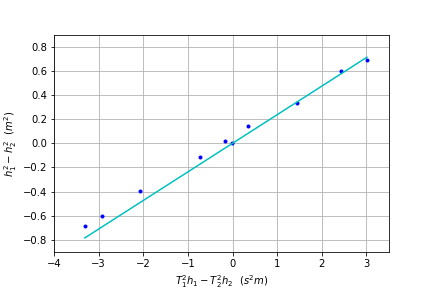
\includegraphics[width=11cm, height=7cm]{Plot1-Kater.png}
\caption{Representación de $h_1^2-h_2^2$ vs $T_1^2h_1-T_2^2h_2$}
\label{fig:Plot1-kater}
\end{figure}

En la gráfica \ref{fig:Plot1-kater} podemos ver que los datos no se acercan mucho a la regresión. Tango g como la gráfica son un desastre: g no se acerca para nada al valor real que todo el mundo sabe, y en la gráfica la mayor parte de los puntos están lejos de la recta. Aunque las razones de esto las extraeremos en el siguiente capítulo, en este solo nos dedicaremos a expresar y analizar los datos que nos dieron, tratando de calcular, en este caso, g.

\section{Conclusiones}

Bien, antes de sacar otras conclusiones primero analizaremos lo mas importante, que es si cumplimos los objetivos que nos propusimos, que en este caso si que lo hemos cumplido, ya que hemos hallado la constante g mediante el uso del péndulo kater. Ahora bien, dicho dato podríamos considerarlo un fallo estrepitoso, ya que 8,55 $\nsim$ 9,81. \\

Ahora deberíamos reflexionar sobre la naturaleza de este fallo. Una de las razones por las que puede existir es que cuando nosotros colgábamos el péndulo del soporte este no solo oscilaba en un sentido, si no que tenía un leve movimiento circular, lo cual es producto del material, ya que en las cuchillas del péndulo una es mas grande que la otra, así como el soporte no deja que las cuchillas se coloquen correctamente. Además otra de las razones de este fallo es que quizás al medir las distancias el metro no mide perfectamente la distacia ya que debido a la forma de las cuchillas es realmente difícil saber donde empieza ya acaba la distancia. Otro problema quizás es que también es difícil medir cual es el punto exacto de G dentro del péndulo. Sin embargo todos estos errores, aun acumulados, no deberían dar un error tan grande, ya que a pesar de que si, influyen mucho en el resultado, si le echamos un vistazo a la gráfica algo no cuadra: \\

Como podemos ver al principio tenemos que los puntos están por encima de la gráfica, muy alineados. Esto se puede deber a que cometimos un error sistemático en estos. En los siguientes no cometimos dicho error, por eso la gráfica está tan distorsionada, y g también. A pesar de que el coeficiente de regresión lineal es bastante bueno, podemos apreciar que no está bien. De hecho si representamos la regresión lineal nuestra con una ideal veríamos que difieren bastante (véase figura \ref{fig:Plot2-kater}). \\

\begin{figure}[h!]
\centering
\includegraphics[scale=0.8]{Plot2-kater.png}
\caption{representación de la regresión lineal vs g=9,81}
\label{fig:Plot2-kater}
\end{figure}

Por lo que puedo concluir que para mejorar la práctica solo habría que repetirla de nuevo, revisando el material y tratando de evitar el error sistemático.  Sin embargo no todo es malo, ya que errar también es parte de los experimentos científicos, y muchas veces los resultados experimentales son necesarios para continuar mejorando. Por esa misma razón no hemos rehecho la práctica, ya que enriquece nuestro conocimiento.


\end{document}
